%% Failure-Routing in AI/ML Python Except-Handlers: Corpus Measurements and
%% Validation Limits
%%
%% Reported counts are derived from committed artefacts in the accompanying
%% repository: the reference-set ledger, the two label sets, the arm-3 closure
%% ledger, and the scan exports under bench/. All are itemised, with commands,
%% in "Reproduction and artefacts". The paper reports descriptive counts.
%%
%% Build (TeX Live): pdflatex main && bibtex main && pdflatex main && pdflatex main
%% Build (single binary, used for the submitted PDF):
%%       tectonic -X compile main.tex --keep-logs --keep-intermediates
%%
\documentclass[10pt,a4paper]{article}

\usepackage[T1]{fontenc}
\usepackage{lmodern}
\usepackage[margin=2.6cm]{geometry}
\usepackage{booktabs}
\usepackage{array}
\usepackage{graphicx}
\usepackage{url}
\usepackage{microtype}
\usepackage{enumitem}
\usepackage{xcolor}
\usepackage{verbatim}
% natbib is loaded for one reason: plainnat, unlike plain, prints the doi/url
% field, so every entry in the reference list becomes resolvable. The numeric
% option keeps the bracketed style this document is written in, and \cite is
% aliased to \citep so that it stays a bare number --- natbib would otherwise
% print "Author [n]" beside author names the running text already supplies.
\usepackage[numbers,sort&compress]{natbib}
\let\cite\citep
% hyperref is loaded last, as it requires. pdfauthor and pdftitle are set
% explicitly so that hyperref need not sanitise the \thanks footnote out of the
% author string when it writes the document metadata.
\usepackage[colorlinks=true,allcolors=blue]{hyperref}
\hypersetup{
  pdfauthor={Yufeiyang Chen},
  pdftitle={Failure-Routing in AI/ML Python Except-Handlers: Corpus Measurements and Validation Limits},
  pdfsubject={Empirical study of except-handler failure-routing in AI/ML Python},
  pdfkeywords={exception handling; silent failure; static analysis; empirical software engineering; machine learning systems}
}
\emergencystretch=2em
\newcolumntype{P}[1]{>{\raggedright\arraybackslash}p{#1}}

% The author footnote states contribution, generative-tool disclosure, and the
% project's evaluation role.
% Keep the title on one metadata-safe line; arXiv indexes it as a single string.
\title{Failure-Routing in AI/ML Python Except-Handlers: Corpus Measurements and Validation Limits}
\author{Yufeiyang Chen\thanks{%
  \textbf{Author contribution.} The author originated the \texttt{failroute}
  idea and directed the study, including its research questions and key decisions.
  AI language tools assisted software development, testing, data analysis, and
  editorial revision. The author takes responsibility for the final work.
  The detector
  and supplementary \texttt{semgrep} rule were developed within this project;
  their evaluation includes results unfavourable to them.
  Corpus labels were produced by LLM agents rather than human annotators; the paper states their provenance and limitations.}\\[2pt]
  School of Cyber Science and Technology, Sun Yat-sen University, Shenzhen, China\\
  \texttt{fei76161@gmail.com}}
% The date is deliberately empty: a submitted PDF must not carry a draft stamp,
% and arXiv records the submission and announcement dates itself.
\date{}

\begin{document}
\maketitle

% The arXiv metadata form accepts at most 1920 characters, and the form is the
% abstract readers actually search, so the text below is what gets pasted into it.
% Convention: the environment's body, stripped of leading and trailing whitespace,
% each newline one character, TeX markup NOT stripped. Do not re-measure by hand and
% do not write the number into this comment -- it is a command now:
%     .venv/bin/python tools/check_abstract_len.py
% The tool measures the source convention used by the arXiv abstract form and
% exits non-zero when either measured form exceeds the configured character limit.
% Keep the body flush-left: indented source makes the raw count include the
% indentation, and the two conventions then diverge by enough to hide an overrun.
% Do not spell the two environment markers literally in this comment -- a matcher
% scanning for them finds the comment first and measures the wrong span.
\begin{abstract}
Exception handlers can turn operational failures into success-shaped values,
such as an LLM judge outage becoming a legitimate \texttt{0.0}. We study this
pattern in eight pinned AI/ML Python packages. \texttt{failroute} 0.8.0 reports
621 candidates over 524,229 scanned lines; 366 are not co-located with the
selected rules of four syntactic linters. Co-location does not establish
equivalent detection, and candidates are not confirmed defects.

A revised predicate reduces the list to 476 findings and raises four-linter
co-location from 41.1\% to 52.9\%. In an exploratory join of 140 LLM-labelled
observations, 104 match that frame: 12 of 48 co-located and 1 of 56
non-co-located observations carry DEFECT labels. The supplementary 60 were
purposively selected and labels are clustered, so this contrast is descriptive. The original 80 labels include
12 DEFECT labels in three repeated function families in one package; five
concern discarded comparisons whose failure-conversion mechanism is
unestablished. All 12 original labels occur among the 134 candidates reported
by \texttt{flake8}'s E722 rule, but this does not confirm the labels or estimate
E722's precision.

Two LLM labelling rounds agree completely, but their independence and accuracy
are unestablished. Thirteen of 478 tracked sites were classified as fixed, and
16 of 43 selected family-fix pull requests were merged. These sources describe
different selected records and do not identify a common defect rate. In a
curated merged-fix set, the detector matches 3 of 14 in-scope cases; nine route
failure outside handlers. The study documents how predicate refinement changes
candidate and co-location counts, while the available evidence does not
establish a change in confirmed-defect yield. Its output is a review queue
requiring adjudication.
\end{abstract}

\section{Introduction}

Many software failures announce themselves. An exception propagates, a process
exits, a stack trace reaches a log. Some failures do none of this. A handler
catches a timeout from a model API and returns \texttt{0.0}, and
the caller cannot distinguish that from a model that genuinely scored zero. A
decode error is caught and an empty string returned, and the code downstream sees
a document with no content rather than one that failed to load. Execution
continues, the caller receives a value of the expected type, and a wrong answer
proceeds in the shape of a right one. We call this \emph{failure-routing}: the
handler does not merely swallow the failure, it routes it into the success path.
This paper studies local exception-handling code: primarily failures routed
inside an \texttt{except} handler, plus the adjacent
\texttt{contextlib.suppress} form. One registered rule concerns exception
masking rather than a success-shaped result; we distinguish it below.

The consequence is that the usual evidence of a defect may be missing by
construction. A crash can produce a bug report; a plausible wrong number may
not. An issue or regression test may never be filed, so the standard warrant for
a static-analysis finding --- that a maintainer read and fixed it --- is least
available for some of the failures this pattern is meant to describe.
Detecting these handlers is the easy half of the problem. Establishing that what
we detected are defects is the hard half, and it is the half we do not fully
solve.

This work began with a narrower observation about Ruff's \texttt{SIM105}
rule: its recommended refactoring can move a handler pattern outside the
detection scope of the selected lint rules studied here.

\paragraph{The \texttt{SIM105} observation.}
\begin{itemize}[nosep,leftmargin=*]
\item \texttt{ruff}'s \texttt{SIM105} rule recommends rewriting a simple
  \texttt{try/except/pass} block with
  \texttt{contextlib.\allowbreak suppress(...)}. In a straightforward rewrite the two
  forms suppress the same specified exception; their behaviour need not be
  identical in every surrounding context.
\item After the rewrite, the construct is out of reach of the linters we tested,
  and not only of the rule sets we happened to select: in our corpus all 19
  \texttt{contextlib.\allowbreak suppress} findings are invisible
  to the union of \texttt{ruff}, \texttt{bandit}, \texttt{pylint} and
  \texttt{flake8}\allowbreak\texttt{+}\allowbreak\texttt{bugbear}, and enabling
  every one of \texttt{ruff}'s 969 rules, or \texttt{pylint}'s full default message
  set, adds no rule that reports it (Section~\ref{sec:rq1}). A \texttt{semgrep}
  project's supplementary rule covers 18 of the 19; citing it requires stating the rule is
  ours.
\item The direct refactoring can preserve the intended suppression behaviour
  while placing the rewritten construct outside the rule sets observed here;
  whether a given instance is defective remains a separate question.
\end{itemize}

\paragraph{Research questions.}
\begin{itemize}[nosep,leftmargin=*]
\item \textbf{RQ1} How many local exception-handling candidates occur in
  the eight pinned AI/ML Python packages, and how often are they co-located with
  findings from the selected syntactic lint rules? (Section~\ref{sec:rq1})
\item \textbf{RQ2} What labels do two LLM-based rounds assign to sampled
  findings, and what do those labels establish about defect status?
  (Section~\ref{sec:rq2})
\item \textbf{RQ3} How many fixes in the curated maintainer-merged reference
  set match the detector, and how many route failure outside an except-handler?
  (Section~\ref{sec:rq3})
\item \textbf{RQ4} What detector change followed review of the sampled labels?
  (Section~\ref{sec:rq4})
\item \textbf{RQ5} How does a revised predicate change the findings and their
  co-location with selected lint rules, and what can the available labels show?
  (Section~\ref{sec:rq5})
\end{itemize}
\paragraph{Contributions.}
\begin{enumerate}[nosep,leftmargin=*]
\item A taxonomy of five silent-continuation or failure-to-value shapes and
  one adjacent exception-masking shape, with an AST detector for them
  (Section~\ref{sec:family}).
\item A reproducible count and cross-tool co-location measurement over eight
  pinned packages (Section~\ref{sec:rq1}).
\item A stratified sample ($n=80$) with LLM labels and an analysis of their
  limitations (Section~\ref{sec:rq2}); the labels do not establish precision
  against independently confirmed defects.
\item A comparison of three differently selected evidence sources
  (Section~\ref{sec:tri}) showing that these data do not identify a common
  defect rate; we specify a future measurement that could address the gap.
\item A comparison with a curated maintainer-merged reference set
  (Section~\ref{sec:rq3}): the detector matches three of fourteen in-scope
  fixes, while nine route failure outside an except-handler.
\item Four sampled findings labelled FALSE POSITIVE shared a control-flow
  shape; the resulting correction removed ten candidates emitted by one rule
  on this corpus (Section~\ref{sec:rq4}).
\item A finite-set comparison of predicate refinement (Section~\ref{sec:rq5}):
  findings fell from 621 to 476, while four-linter co-location rose from 41.1\%
  to 52.9\%. In 104 joined, selected observations, 12 of 48 co-located and 1
  of 56 non-co-located records carried LLM DEFECT labels. The labels are
  clustered and the supplementary records were purposively selected, so this
  contrast does not establish which group contains more defects.
\item A simple baseline comparison: \texttt{flake8 --select E722} returns 134
  candidates and includes all 12 original DEFECT-labelled observations in the
  sample. This is a finite label-set comparison, not an estimate of E722's
  precision or coverage of confirmed defects (Section~\ref{sec:rq1}).
\end{enumerate}

\section{The pattern family}
\label{sec:family}

The six registered shapes are listed in Table~\ref{tab:shapes}. Five concern a
caught failure that is suppressed or routed into a normal-looking value or
continuation. \texttt{name-shadowing} is different: it can replace the original
exception with a \texttt{NameError}, masking the cause without producing a
success-shaped value. We include it as an adjacent exception-handling hazard,
not as evidence of silent success. The taxonomy is defined by the semantics of
the Python constructs involved rather than fitted
to the corpus studied here: four of the six shapes account for all 621 findings
reported in Section~\ref{sec:rq1}, and the two that never fire on this corpus are
retained because a shape's absence from one corpus is not evidence that the shape
does not occur. Both are exercised by the tool's unit corpus.

\begin{table}[htbp]
\centering\small
\caption{Five silent-continuation or failure-to-value shapes and one adjacent
exception-masking shape.}
\label{tab:shapes}
\begin{tabular}{@{}P{3.0cm}P{5.3cm}P{6.0cm}@{}}
\toprule
Rule & Shape & Consequence \\
\midrule
\texttt{no-action} & \texttt{except ...: pass} & handler emits no direct
failure signal \\
\texttt{silent-fallback} & handler returns/assigns a constant without re-raising
& judge outage becomes a legitimate \texttt{0.0} \\
\texttt{masked-exception} & catch-all conditionally re-raises \emph{and} falls
back to a constant & outcome depends on which branch ran \\
\texttt{silent-suppress} & \texttt{with contextlib.suppress(...)} & suppresses
specified exceptions; invisible to the linters we tested \\
\texttt{implicit-fallback} & handler neither re-raises, returns, nor records ---
falls through to implicit \texttt{None} & ``did nothing'' becomes a legitimate
\texttt{None} \\
\texttt{name-shadowing} & \texttt{except E as e:} rebinds \texttt{e} inside the
handler & Python deletes the binding on exit; a later use can raise
\texttt{NameError} or \texttt{UnboundLocalError} \\
\bottomrule
\end{tabular}
\end{table}

\section{The detector}
\label{sec:detector}

The tool is the instrument, not the subject, so we describe it only to the extent
needed to interpret the study. \texttt{failroute} 0.8.0 parses each file to an
AST and applies six rules through a shared registry, emitting text, JSON or
SARIF; individual rules can be disabled per project under
\texttt{[tool.failroute]}.

\paragraph{Unit of analysis.} One finding is one \texttt{except} handler --- or,
for the \texttt{silent-suppress} rule, one \texttt{contextlib.suppress}
statement --- reported at the line where it starts. Findings are sorted by line,
with a stable per-handler registry order for findings that share a line, so the
output order is deterministic.

\paragraph{What counts as silence.} The tool treats a failure as explicitly
signalled, rather than silently routed, if its handler re-raises; calls
\texttt{exit} or \texttt{\_exit}; calls \texttt{warnings.warn} or
\texttt{warnings.warn\_explicit}; or calls a logger-like name. Two properties of
that test matter for reading Section~\ref{sec:rq2}.

First, the test is \emph{not} uniform across handler kinds. A \textbf{catch-all}
handler (bare \texttt{except:} or \texttt{except Exception:}) must call a method
named in \{error, warning, warn, exception, critical, fatal\}; a \textbf{typed}
handler qualifies on \emph{any} method of a logger-like object, \texttt{debug} and
\texttt{info} included --- and, because the test matches the object rather than the
method's meaning, on method names that are not logging calls at all.
\texttt{capture\_exception} on a logger-like object also qualifies. A bare
\texttt{print()} never does. Thus \texttt{logger.debug()} prevents a finding
for a typed handler under this syntactic test but not for a catch-all handler. The asymmetry is
deliberate: a typed clause documents the failure its author anticipated. It
does not establish that a debug message reaches the caller.
Section~\ref{sec:rq5} shows the asymmetry matters in this sample: every
original LLM DEFECT label sits on a bare handler, which falls through the
strict half of this test rather than the lenient half.

Second, the test is not global. Only \texttt{silent-fallback} and
\texttt{implicit-fallback} consult it; \texttt{no-action},
\texttt{masked-exception} and \texttt{name-shadowing} report without asking whether
the handler recorded anything.

``Logger-like'' means a base-name list
(\texttt{logger}, \texttt{logging}, \texttt{log}, \texttt{\_logger},
\texttt{\_log}, \texttt{sentry\_sdk}) plus a suffix heuristic, since real
codebases name loggers \texttt{audit\_logger}, \texttt{err\_log} and
\texttt{self.\_log}. Handler bodies are traversed through control flow but
\emph{not} into nested function, lambda or class bodies, so a \texttt{return None}
inside a callback defined in a handler does not silence it.

\paragraph{What counts as a fallback value.} A fixed constant set
(\texttt{None}, \texttt{False}, \texttt{0}, \texttt{0.0}, \texttt{""},
\texttt{[]}, \texttt{\{\}}, \texttt{()}), whose ambiguous members
(\texttt{True}, \texttt{1}, \texttt{1.0}) are marked as such because they are
legitimate in boolean scorers, plus namespace-qualified sentinels such as
\texttt{Status.UNKNOWN} and any project-specific values configured under
\texttt{[tool.failroute]}. Bare names are deliberately not matched, so
\texttt{return result} can never fire.

\paragraph{Exemptions.} Three gates remove a site before any rule runs. The
first is the caught type. A handler catching only \texttt{KeyboardInterrupt},
\texttt{SystemExit} or \texttt{GeneratorExit} is exempt. The same applies to
\texttt{StopIteration}, \texttt{StopAsyncIteration} or
\texttt{CancelledError}; a tuple handler is exempt only when every member is.
These exceptions can occur in
shutdown, iteration and cancellation handling, where suppression may be
intentional; the tool does not determine whether it is appropriate at a given
site. The exemption can therefore also hide a genuine mistake. The second gate
is an opt-out marker in the handler's own lines:
\texttt{\# failroute: ignore} or \texttt{\# pragma: no cover}. The third is
configuration: a rule disabled under \texttt{[tool.failroute]} never fires. All
three gates are applied once, in the dispatcher, rather than re-implemented per
rule.

The heuristics deliberately err on the side of reporting: a finding is meant to
be worth a look, not to be a verdict. Section~\ref{sec:rq2} reports LLM labels
for a sample; those labels do not measure precision against confirmed defects.

\paragraph{Quality gates.} The v0.8.0 release has 158 tests and a CI matrix
covering Ubuntu, macOS and Windows with Python 3.9--3.13, plus
\texttt{mypy --strict}. Its v6 unit-fixture corpus contains 36 positive and 32
negative cases; CI checks each against its expected result.

\paragraph{Construct validity.} Fixture agreement shows that the detector
implements its tested specification; it does not show that its findings are
real defects. Section~\ref{sec:rq2} is a limited within-corpus label audit,
not an external validation against confirmed defects.

\section{Study}
\label{sec:study}

\paragraph{Statistical reporting.}
The paper reports finite-set counts and descriptive proportions. The weighted
RQ2 projection estimates the number of LLM DEFECT labels in its corrected
sampling frame; it is not an estimate of confirmed defects. The package,
co-location, and PR comparisons have different sampling or selection processes
and are not used to infer population rates or causal effects. No confidence
intervals are reported because the available labels and selected records do not
support the population claims such intervals might suggest.

\subsection{Corpus}
\label{sec:corpus}

Eight AI/ML packages fetched as pinned PyPI source distributions (not git
clones), each recorded with URL, SHA-256, upload time and extracted tree hash in
\texttt{paper/corpus-lock.json}. Table~\ref{tab:corpus} lists them. Together the
eight sdists hold 2{,}354 \texttt{.py} files and 563{,}270 lines; the scan roots the
detector actually reads hold 2{,}124 files and 524{,}229 lines; finding-density
figures are calculated over those scan roots. Fetching is pinned rather than
merely scripted: \texttt{tools/fetch\_corpus.py} resolves each package to the
version recorded in \texttt{paper/corpus-manifest.json}, checks the downloaded
archive's SHA-256 against the same manifest, and exits non-zero on mismatch, so a
re-fetch either reproduces these inputs or fails loudly. A fresh fetch into a
clean directory on 2026-09-02 reproduced all eight archives byte-identically (8/8
SHA-256 matches against \texttt{corpus-lock.json}).

\begin{table}[htbp]
\centering\small
\caption{Pinned corpus. Per-package counts are the files \emph{inside each scan
root} --- the subtree the detector actually scans --- so the column sums to the
total shown (2{,}124 \texttt{.py} files / 524{,}229 lines). The eight pinned
sdists contain \textbf{2{,}354} \texttt{.py} files / \textbf{563{,}270} lines in
total; the difference is content outside the scan roots (tests, examples,
vendored code).}
\label{tab:corpus}
\begin{tabular}{@{}lllrr@{}}
\toprule
Package & Version & Scan root & \texttt{.py} files & Lines \\
\midrule
inspect\_ai & 0.3.260 & \texttt{src/inspect\_ai} & 755 & 198{,}351 \\
pydantic\_ai\_slim & 2.36.0 & \texttt{.} & 298 & 119{,}534 \\
deepteam & 1.0.9 & \texttt{deepteam} & 588 & 71{,}305 \\
trl & 1.12.0 & \texttt{trl} & 155 & 65{,}727 \\
garak & 0.16.0 & \texttt{garak} & 201 & 38{,}328 \\
smolagents & 1.26.0 & \texttt{src/smolagents} & 20 & 13{,}355 \\
uqlm & 0.6.5 & \texttt{uqlm} & 91 & 12{,}605 \\
fickling & 0.1.12 & \texttt{fickling} & 16 & 5{,}024 \\
\midrule
\textbf{Total (scanned)} & & & \textbf{2{,}124} & \textbf{524{,}229} \\
\bottomrule
\end{tabular}
\end{table}

A second, style-opposite corpus tests whether the headline comparison survives outside bare-\texttt{except} code. Eight infrastructure packages were fetched as pinned PyPI sdists (URL, SHA-256, upload time and tree hash in \texttt{paper/corpus-lock-control.json}, same schema as above): \texttt{attrs} 26.1.0, \texttt{httpx} 0.28.1, \texttt{requests} 2.34.2 and \texttt{urllib3} 2.7.0 (the four zero-bare-\texttt{except} packages of Section~\ref{sec:control}), plus \texttt{click} 8.5.0 (CLI), \texttt{pydantic} 2.13.5 (validation), \texttt{anyio} 4.15.1 (concurrency) and \texttt{msgpack} 1.2.2 (serialization) --- chosen for domain diversity before any scan ran, explicitly avoiding the HTTP-client stack that three of the first four share. Only each package body is scanned (scan roots recorded in the lock file), the same definition as above. Section~\ref{sec:control} reports the comparison.

\subsection{RQ1 --- Corpus counts and cross-tool co-location}
\label{sec:rq1}

\texttt{failroute} (v0.8.0) reports \textbf{621} findings. Baselines were run on
the \emph{same} pinned trees; Table~\ref{tab:tools} lists the tools, their
versions and the rule sets they were invoked with.

\paragraph{Matching protocol.} Each baseline was invoked with only the rules that
address this family --- \texttt{ruff} S110/S112, \texttt{bandit} B110/B112,
\texttt{pylint} W0702/W0703/W0705/W0706, \texttt{flake8} E722 with
\texttt{bugbear} B001/B017 --- and every report was reduced to a (file, line)
pair. A \texttt{failroute} finding counts as \emph{covered} by a baseline when
that baseline reported any of its selected rules in the same file within $\pm$1
line of it (\texttt{TOL $=$ 1} in \texttt{tools/coverage\_union.py}), and as
covered by the \emph{union} when any baseline covers it. Co-location is
deliberately a weak criterion --- it asks whether a tool flagged the same
handler, not whether it expressed the same property --- and the caveat at the end
of this subsection states what that costs.

\paragraph{A blind spot in the baseline harness and its correction.}
The initial harness passed each scan root to \texttt{pylint} as a single directory
argument. \texttt{pylint} walks a directory as a \emph{package}
and does not descend into one with no \texttt{\_\_init\_\_.py}, so every module
under such a directory is silently never analysed --- no message, no error, exit 0.
Here 152 of the 2{,}124 scanned files (7.2\%) sit under one (\texttt{inspect\_ai}
123, \texttt{deepteam} 20, \texttt{garak} 9), and RQ1's exact selection emits 34
messages across 20 of them that the directory invocation reported as zero. Handing
\texttt{pylint} the file list recovers them and perturbs nothing else: on the files
it already reached, the two invocations agree message for message (0 lost, 0
gained, per package), so the correction is a pure addition to the baseline. Every
figure in this paper uses the corrected invocation, and it moves the four-linter
union from 250 to 255 of 621 and \texttt{failroute}-only from 371 to 366 --- it
\emph{reduces} the detector's measured novelty, which is the direction a
self-inflicted error should be reported in. The other three baselines have no
equivalent blind spot: \texttt{ruff}, \texttt{bandit} and \texttt{flake8} are
filesystem walkers, and over those same 152 files their directory and
explicit-file invocations return identical hit sets --- 6{,}879 messages under
\texttt{ruff\ --select\ ALL}, 104 under \texttt{bandit} with every test enabled,
and 2{,}375 under \texttt{flake8}'s default selection, identical both ways. Under
RQ1's own narrow selections those same files yield 5, 0 and 0, which is why the
blind spot cost only \texttt{pylint} anything. The control corpus of
Section~\ref{sec:control} contains no \texttt{\_\_init\_\_}-less directory at all
(0 of 263 files), so it was never exposed. \texttt{--recursive=y} and
\texttt{--init-hook} were both tested; neither recovers a single message.

One asymmetry in that rule list we disclose rather than defend: \texttt{pylint} is
granted W0703 (broad \texttt{except}), whose direct \texttt{ruff} analogue BLE001
was \emph{not} selected, so \texttt{ruff} was the only baseline denied its
broad-except rule. Re-running with BLE001 added, \texttt{ruff}'s \emph{own}
co-located findings rise from 72 to 127 (410 findings in total rather than 76),
but the four-tool union does not move: 255 of 621 and \texttt{failroute}-only 366
under either selection, because every finding BLE001 newly reaches is one
\texttt{pylint}'s W0718 already reaches. \texttt{silent-suppress} stays at 0/19
either way, since BLE001 fires on \texttt{except} clauses and the shape in
question has none. The asymmetry therefore costs the union nothing and bears only
on the per-tool comparison below; we keep the narrower selection as the headline
because that is what the publicly tagged artefact set reproduces. The symmetric run
is \texttt{tools/coverage\_union.py --ruff-select S110,S112,BLE001}, and its output
is committed as \texttt{bench/corpus-coverage-union-ruff-ble001.json}.

\begin{table}[htbp]
\centering\small
\caption{Cross-tool comparison on the pinned corpus. The \texttt{semgrep} row is
\emph{not} a shipped-rule baseline: its rule set
(\texttt{tools/semgrep-rules/exception-handling.yaml}) was written by us, so it
shows what a syntactic-pattern engine \emph{can} express given rules, not what
users get by default. $+19$ is the number of \texttt{failroute} findings newly
co-located once \texttt{semgrep} is added to the union (mostly the
\texttt{contextlib.suppress} shape: 18 of 19). Versions are those installed in the
reproduction environment and are the versions that produced the committed
artefacts. Three provenance notes. \texttt{pyproject.toml} pins
\texttt{ruff==0.16.5}, one patch above the 0.16.4 that produced the committed
artefact; 0.16.0, 0.16.4 and 0.16.5 all produce \emph{set-identical} hits for both
rule selections (76 findings and 72 co-located for S110/S112; 410 and 127 for
S110/S112/BLE001), so the row is stable across every patch release we can install.
The \texttt{pylint} \emph{Findings} cell is the one count in this table that
depends on the analysis environment rather than on the corpus: \texttt{pylint}
resolves imported names, so a handler that re-raises before a later
\texttt{except Exception} is correctly left alone when the caught type is
importable and reported as \texttt{W0706} when it is not. With \texttt{click}
present, \texttt{pylint} reports 563 findings; without \texttt{click}, as in the
documented install, it reports 564 and the hidden-file count above reads 35 across 21. Table~\ref{tab:tools}
gives these values in that order.
Co-location is unaffected --- 255, and identical rule by rule, either way --- so no
figure in this paper moves. And \texttt{semgrep} does not appear in
\texttt{pyproject.toml} at all: the five-tool row is a frozen artefact
(\texttt{bench/corpus-coverage-union-5tool.json}), not a step the documented
install reproduces. Its generator, \texttt{tools/run\_semgrep\_baseline.py}, reads
the v0.7.0 frame and writes over that artefact, so it reproduces neither the row
nor the file: do not run it against the committed export.}
\label{tab:tools}
\begin{tabular}{@{}lllrr@{}}
\toprule
Tool & Version & Rules & Findings & Co-located $\pm$1 line \\
\midrule
\textbf{\texttt{failroute}} & 0.8.0 & all six & \textbf{621} & --- \\
\texttt{ruff} & 0.16.4 & S110, S112 & 76 & 72 \\
\texttt{bandit} & 1.9.4 & B110, B112 & 67 & 63 \\
\texttt{pylint} & 4.0.8 & W0702, W0703, W0705, W0706 & 563/564 & 255 \\
\texttt{flake8}+\texttt{bugbear} & 7.3.0 / 25.11.29 & E722, B001, B017 & 268 & 124 \\
\texttt{semgrep} (our rules) & 1.175.0 & hand-written, 6 shapes & --- & $+19$ \\
\bottomrule
\end{tabular}
\end{table}

\textbf{The four selected syntactic linter rule sets co-locate with 255 of 621
findings (41.1\%); 366 (58.9\%) have no such co-location.} Adding our
\texttt{semgrep} rules raises the co-located count to 274 (44.1\%) and lowers the
unmatched count to 347 (55.9\%). These are exact corpus counts under the stated
matching rule, not estimates of equivalent detection. Table~\ref{tab:coverage}
breaks them down by rule and Figure~\ref{fig:coverage} plots them.

\begin{table}[htbp]
\centering\small
\caption{Per-rule co-location counts under the stated $\pm$1-line criterion.
The four-tool union includes \texttt{ruff}, \texttt{bandit}, \texttt{pylint},
and \texttt{flake8} with \texttt{bugbear}; the next column adds the project's
supplementary \texttt{semgrep} rule. The two zero-count families remain in the
detector but do not occur in this corpus. For \texttt{silent-suppress}, none of
the selected rules, nor the full \texttt{ruff} and \texttt{pylint} rule sets,
reports a relevant warning on the 19 findings; the project rule co-locates with
18.}\
\label{tab:coverage}
\begin{tabular}{@{}lrrrr@{}}
\toprule
Rule & Findings & Four-tool union & With semgrep & Not co-located with four \\
\midrule
\texttt{silent-fallback} & 386 & 180 & 181 & 206 \\
\texttt{no-action} & 213 & 72 & 72 & 141 \\
\textbf{\texttt{silent-suppress}} & \textbf{19} & \textbf{0}
& \textbf{18} & \textbf{19} \\
\texttt{masked-exception} & 3 & 3 & 3 & 0 \\
\texttt{implicit-fallback} & 0 & --- & --- & --- \\
\texttt{name-shadowing} & 0 & --- & --- & --- \\
\bottomrule
\end{tabular}
\end{table}

\begin{figure}[htbp]
\centering
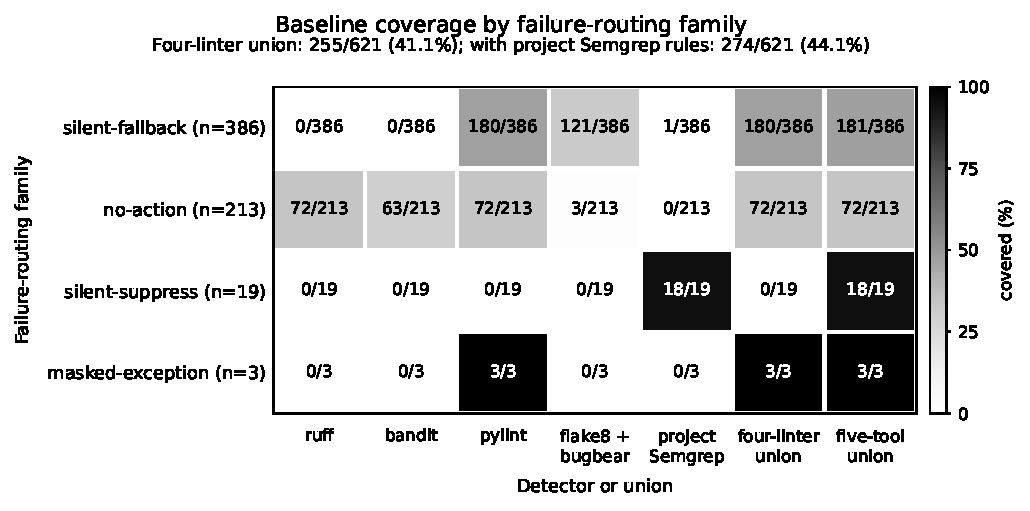
\includegraphics[width=\textwidth]{figures/fig2_cross_tool_coverage.pdf}
\caption{Coverage of the 621 pinned findings by rule family and detector. Each
cell gives covered findings / family total; shading encodes the coverage share.
The four-linter union covers 255/621 findings; adding the project's supplementary
\texttt{semgrep} rules covers 274/621. \texttt{silent-suppress} is the one family
where the four linters, \texttt{ruff}'s full 969-rule set and \texttt{pylint}'s full
default set all return zero coverage.}
\label{fig:coverage}
\end{figure}

\paragraph{Two observations that cut against the tool.}
\begin{enumerate}[nosep,leftmargin=*]
\item \texttt{pylint} is a stronger baseline than \texttt{ruff}, by a factor that
  depends on which \texttt{ruff} rules the comparison allows. Against
  \texttt{ruff}'s S110/S112 alone, the gap is 3.54$\times$ (72 vs 255
  co-located findings). Adding \texttt{ruff}'s broad-except rule BLE001, symmetric
  to the W0703 \texttt{pylint} rule, reduces the gap to 2.01$\times$ (127 vs
  255). The comparison depends on the stated rule selection; we report both
  rather than treating the narrower one as representative of \texttt{ruff}'s
  broad-except coverage.
\item \texttt{masked-exception} is fully covered. All 3 findings co-locate with a
  \texttt{pylint} broad-except warning. That rule contributes no coverage novelty
  here; this finite count is specific to the pinned corpus.
\end{enumerate}

\paragraph{A simple baseline for candidate-list length.}
The union above asks which detector findings a linter flags near the same line; it
does not compare candidate-list lengths. Across the same eight scan roots,
\texttt{flake8 --select E722} reports \textbf{134} bare-except candidates,
including all \textbf{12} original LLM DEFECT-labelled sites. Its list is
4.63$\times$ shorter than the 621-finding v0.8.0 list and 3.55$\times$ shorter
than the 476-finding refactored list. These are list-size comparisons at equal
coverage of the twelve original labels, not equal recall of confirmed defects.
The sample was drawn from \texttt{failroute} findings, not from E722's candidate
list, so it cannot estimate E722's label yield or precision.

\texttt{ruff}'s broad-except rule BLE001 is a useful contrast: it returns 334
candidates and co-locates with none of the 12 original LLM DEFECT-labelled
sites. BLE001 fires on \texttt{except Exception:}, not bare \texttt{except:};
all 12 labels in the frozen sample are attached to bare handlers. This is a
finite overlap result, not evidence that E722 detects confirmed defects better
than BLE001.

Both counts come from \texttt{tools/e722\_baseline.py}, which fails loudly if
either linter is unusable rather than reporting an empty hit set, and are
committed as \texttt{bench/e722-baseline.json}.

\paragraph{Methodological caveat on co-location.}
Co-location at $\pm$1 line means that a selected lint rule flags the same
handler; it does not show that the warning expresses the failure-routing
property studied here. A broad-except warning can co-locate for a different
reason. We therefore report the 255/621 co-location count as such and do not
infer semantic coverage or novelty from it.

\subsection{RQ2 --- What do the LLM labels say about sampled findings?}
\label{sec:rq2}

\paragraph{Method.}
We drew a stratified random sample across (rule $\times$ package), with fixed
seed 20260831, at least one draw per stratum, and proportional allocation of the
remaining draws; the sample contains $n=80$ findings. The draw came from an
earlier 659-candidate export. Review then identified ten false-positive
\texttt{implicit-fallback} findings, leaving a 649-candidate corrected frame;
the four sampled findings from that rule were all false positives and are not
included in the frame projection below. Weighting the remaining 76 observations
by stratum size gives a projection of 130 LLM DEFECT labels (20.0\%) in the
649-candidate frame. This is a projection of labels, not confirmed defects, and
we make no claim about confirmed-defect prevalence. The 28 further precision fixes that produced
the v0.8.0 frame removed four additional sampled CONTRACT findings; only 72 of
the original 80 labels remain in that frame, and this surviving subset is not
representative of the current 621-finding set.

The unweighted 12/80 share describes only the drawn sample. Each sampled finding
was assigned one of three labels by reading nearby source in the pinned tree:
\textbf{DEFECT} (the converted failure produces a wrong caller-visible outcome
with no signal), \textbf{CONTRACT} (the behavior appears deliberate and is
documented, commented, or expressed in the return type), or \textbf{FALSE
POSITIVE} (the detector is wrong about the code).

\paragraph{Labelling was performed by LLM agents.}
Two rounds were run, both by LLM agents (not human raters), and they agreed on
80/80 items. This agreement is compatible with shared model bias; it does not
establish label accuracy or independence. The artefacts establish two separate
runs, not independent human adjudication. What
is committed is both label sets --- \texttt{paper/annotations.csv} (first round,
rationales recorded in Chinese) and
\texttt{paper/annotations-second-pass.csv} (second round, rationales in English)
--- so the agreement can be checked item by item rather than taken on trust. The
sample remains useful as (a) a debugging instrument (Section~\ref{sec:rq4}) and
(b) the consequence arm of the triangulation in Section~\ref{sec:tri}, where its
limits are part of the design.

\paragraph{Meaning of a DEFECT label.}
DEFECT denotes the frozen LLM judgement, not an independently confirmed
failure-routing mechanism. Five of the twelve original labels concern a
discarded comparison and an unassigned state; their failure-conversion
mechanism is unestablished. The other seven have the mechanisms described in
Section~\ref{sec:threats}. We retain the original labels for reproducibility;
they do not establish defect yield.

\paragraph{Result (80 sampled findings, LLM-labelled).} Table~\ref{tab:rq2}
reports the sample labels; Tables~\ref{tab:byrule} and~\ref{tab:bypackage}
show their distribution by rule and package. All counts describe this sample;
they do not establish a package-level or corpus-wide defect rate.

\begin{table}[htbp]
\centering\small
\caption{LLM-assigned labels in the original 80-finding sample. Frequencies
describe this sample and are not a defect-rate estimate.}
\label{tab:rq2}
\begin{tabular}{@{}lrr@{}}
\toprule
LLM label & $n$ & Share of sample \\
\midrule
CONTRACT & 64 & 80.0\% \\
DEFECT & 12 & 15.0\% \\
FALSE POSITIVE & 4 & 5.0\% \\
\bottomrule
\end{tabular}
\end{table}

\begin{table}[htbp]
\centering\small
\caption{LLM labels by detector rule in the 80-finding sample. All twelve
DEFECT labels are in \texttt{silent-fallback}; all four FALSE POSITIVE labels
are in \texttt{implicit-fallback}.}
\label{tab:byrule}
\begin{tabular}{@{}lrrrr@{}}
\toprule
Rule & $n$ & DEFECT & CONTRACT & FALSE POS. \\
\midrule
\texttt{silent-fallback} & 49 & 12 & 37 & 0 \\
\texttt{no-action} & 23 & 0 & 23 & 0 \\
\texttt{implicit-fallback} & 4 & 0 & 0 & \textbf{4} \\
\texttt{silent-suppress} & 3 & 0 & 3 & 0 \\
\texttt{masked-exception} & 1 & 0 & 1 & 0 \\
\bottomrule
\end{tabular}
\end{table}

\begin{table}[htbp]
\centering\small
\caption{LLM labels by package in the original 80-finding sample. All twelve
DEFECT labels are in \texttt{deepteam}; all four FALSE POSITIVE labels are in
\texttt{implicit-fallback}. Counts are descriptive of this sample.}
\label{tab:bypackage}
\begin{tabular}{@{}lrrrr@{}}
\toprule
Package & $n$ & DEFECT & CONTRACT & FALSE POS. \\
\midrule
\textbf{deepteam} & 14 & \textbf{12} & 1 & 1 \\
inspect\_ai & 41 & 0 & 40 & 1 \\
pydantic\_ai\_slim & 11 & 0 & 10 & 1 \\
trl & 4 & 0 & 4 & 0 \\
garak & 3 & 0 & 3 & 0 \\
fickling & 3 & 0 & 2 & 1 \\
smolagents & 2 & 0 & 2 & 0 \\
uqlm & 2 & 0 & 2 & 0 \\
\midrule
\emph{all but deepteam} & 66 & \textbf{0} & 63 & 3 \\
\bottomrule
\end{tabular}
\end{table}

\begin{figure}[htbp]
\centering
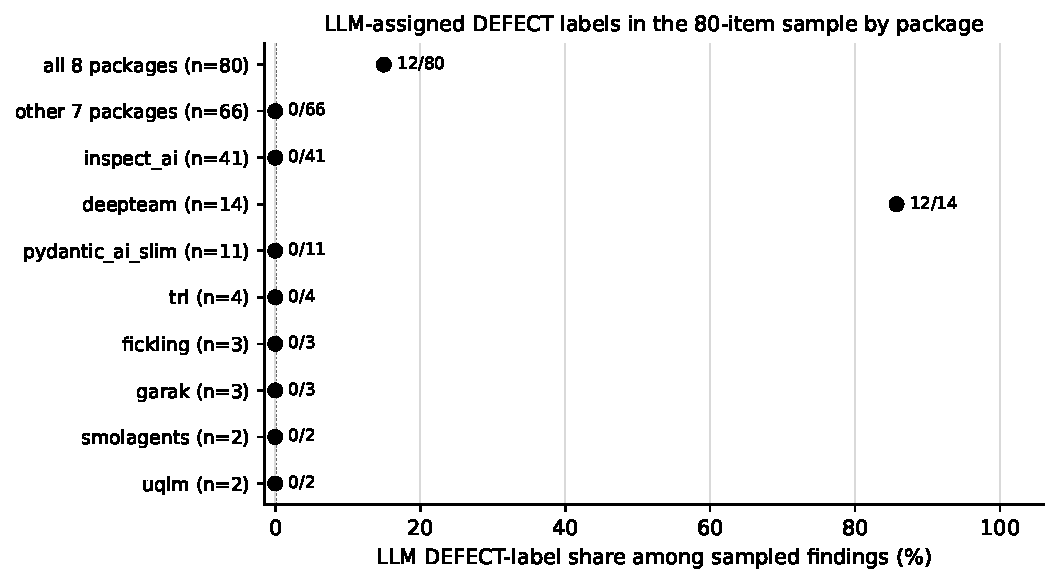
\includegraphics[width=\textwidth]{figures/fig1_llm_label_share_by_package.pdf}
\caption{Share of sampled records assigned the LLM DEFECT label by package.
The plotted shares and counts describe the 80-item sample; they are not
package-level defect-rate estimates.}
\label{fig:defectrate}
\end{figure}

\textbf{All 12 DEFECT labels are in \texttt{deepteam}; none of the 66 sampled
findings from the other seven packages carried that label.} These are sample
counts, not evidence that the other packages have zero defects.

The 12 DEFECT-labelled sites are not 12 independent observations: they fall
into three repeated code families:
\begin{enumerate}[nosep,leftmargin=*]
\item \textbf{Silent criteria degradation (4/12).} A handler catches an error
from \texttt{model.get\_system\_}\allowbreak\texttt{prompt()} and assigns an empty string. If a
custom or misconfigured model lacks that method, later evaluations may run
without the intended criteria. The author's issue on this pattern predates the
LLM labelling pass; it is not independent validation of the label.
\item \textbf{Discarded comparison (5/12).} A handler evaluates
\texttt{self.score == 1} but discards the result, then assigns
\texttt{self.success = False}. The conversion mechanism is unestablished: the
observed score values did not raise, although attribute access or overloaded
equality can raise for other objects.
\item \textbf{Potentially fail-open security verdict (3/12).} A handler catches
an error while iterating results and returns \texttt{vulnerable = False}. In a
red-teaming tool, this could turn an operational failure into a false
\texttt{not vulnerable} result; this interpretation remains an LLM label, not
an independent adjudication.
\end{enumerate}

\paragraph{Handler forms in the labelled sample.}
The 80 sampled findings include 13 bare \texttt{except:} handlers; 12 carry
DEFECT labels. The remaining forms are 18 \texttt{except Exception:}
handlers, 46 narrowly typed handlers, and 3 \texttt{contextlib.suppress}
sites; none in these groups carries an original DEFECT label. These counts are
descriptive of the sample. The three findings in the suppress group are too few
to support a useful comparison, and all labels retain the limitations above.

\paragraph{Sensitivity to repeated findings.}
The twelve original DEFECT labels come from three repeated function families.
The unit used to group copies changes the descriptive share: grouping by package
and enclosing function gives 3 of 68 groups (4.4\%); grouping by exact
signature gives 5 of 71 (7.0\%); grouping by package, file, and function gives
12 of 78 (15.4\%), because copies in separate files remain separate groups.
No one grouping is established as the correct independent unit. These
sensitivity counts reinforce that the 12/80 observation-level share is not a
confirmed-defect rate, and the 20.0\% stratum-weighted projection does not
correct for within-family repetition.

The 64 CONTRACT labels include TUI widget lookups that may not be mounted,
optional-dependency probes, idempotent cleanup in \texttt{finally}, and
predicate functions whose \texttt{Optional}/\texttt{bool} return type is part
of the contract. Some have comments that state the intended fallback; the label
itself remains an LLM judgement.



Two sampled \texttt{pydantic-ai} handlers illustrate why local shape alone is
insufficient: one returns \texttt{True} for an unparseable address, while
another places a caught exception on a queue for the consumer to re-raise.

\subsection{RQ3 --- Reference-set match and construct scope}
\label{sec:rq3}

A curated reference set of upstream fixes in this defect family is available;
the projects' maintainers reviewed and merged those changes. This is not an
exhaustive defect census or an independent adjudication of every merge. Of the 75 pull requests
submitted from the author's account that were merged \emph{as of the 2026-09-01
measurement freeze}, \textbf{16} are failure-routing fixes --- every
exclusion adjudicated by reading the PR diff (52 earlier title-only judgements
were re-checked against diffs in a dedicated pass; 49 stood, 3 flipped). For
each family fix, the file was fetched at the merge commit's \emph{first parent}
(i.e.\ immediately pre-fix) and scanned. Table~\ref{tab:recall} classifies the
16, and every pull request is cited with its repository owner so that the
classification can be checked against the public record.

\begin{table}[htbp]
\centering\footnotesize
\caption{Classification of the 16 family fixes
(\texttt{paper/merged-pr-recall.csv}, all rows diff-read). ``Handler-shape gap''
means design-reachable: a shape outside the current six that could be expressed
without changing the handler-level design.}
\label{tab:recall}
\begin{tabular}{@{}rlP{9.9cm}@{}}
\toprule
Class & $n$ & Cases \\
\midrule
Out of scope for recall & 2 &
\texttt{microsoft/PyRIT\#2460}, a TypeScript-side change (language scope);
\texttt{cvs-health/uqlm\#418}, a pure-additive \emph{Python} fix whose pre-fix
defect is a non-handler implicit-\texttt{None} contract violation the six rules
do not cover by design \\
\textbf{Detected} & \textbf{3} &
\texttt{cvs-health/uqlm\#450},
\texttt{Ishannaik/agent-sweep\#197},
\texttt{truera/trulens\#2653} \\
Handler-shape gap & 2 &
\texttt{UKGovernmentBEIS/inspect\_ai\#5068} (post-handler state
mutation), \texttt{\#4906} (\texttt{tenacity} RetryError masking) --- both
adjudicated as candidate patterns, not shipped \\
\textbf{Non-handler routing} & \textbf{9} & NaN values reaching aggregates,
silently filtered lists, branch-level \texttt{Score(0.0)} returns,
implicit-\texttt{None} contract violations, silently stripped characters,
silently dropped symbols, laundered verdicts \\
\bottomrule
\end{tabular}
\end{table}

\textbf{In the curated reference set, the detector matches 3 of 14 in-scope
fixes (21.4\%).} At most 5 of 14 (35.7\%) use a handler shape potentially
reachable by this detector; nine of 14 (64.3\%) route failure outside an
except-handler. This is coverage of the curated set, not a population recall
estimate.
Figure~\ref{fig:reference-matches} plots the split by defect family.

This is the construct-scope result for the curated reference set. It shows that
the failure-routing cases in that set include patterns outside the local
exception-handling subfamily this tool operationalises. We state this as a
boundary \emph{and} a roadmap --- dataflow-shaped failure-routing is future
work --- and scope the detector's results to handlers and
\texttt{contextlib.suppress} sites accordingly.

\begin{figure}[htbp]
\centering
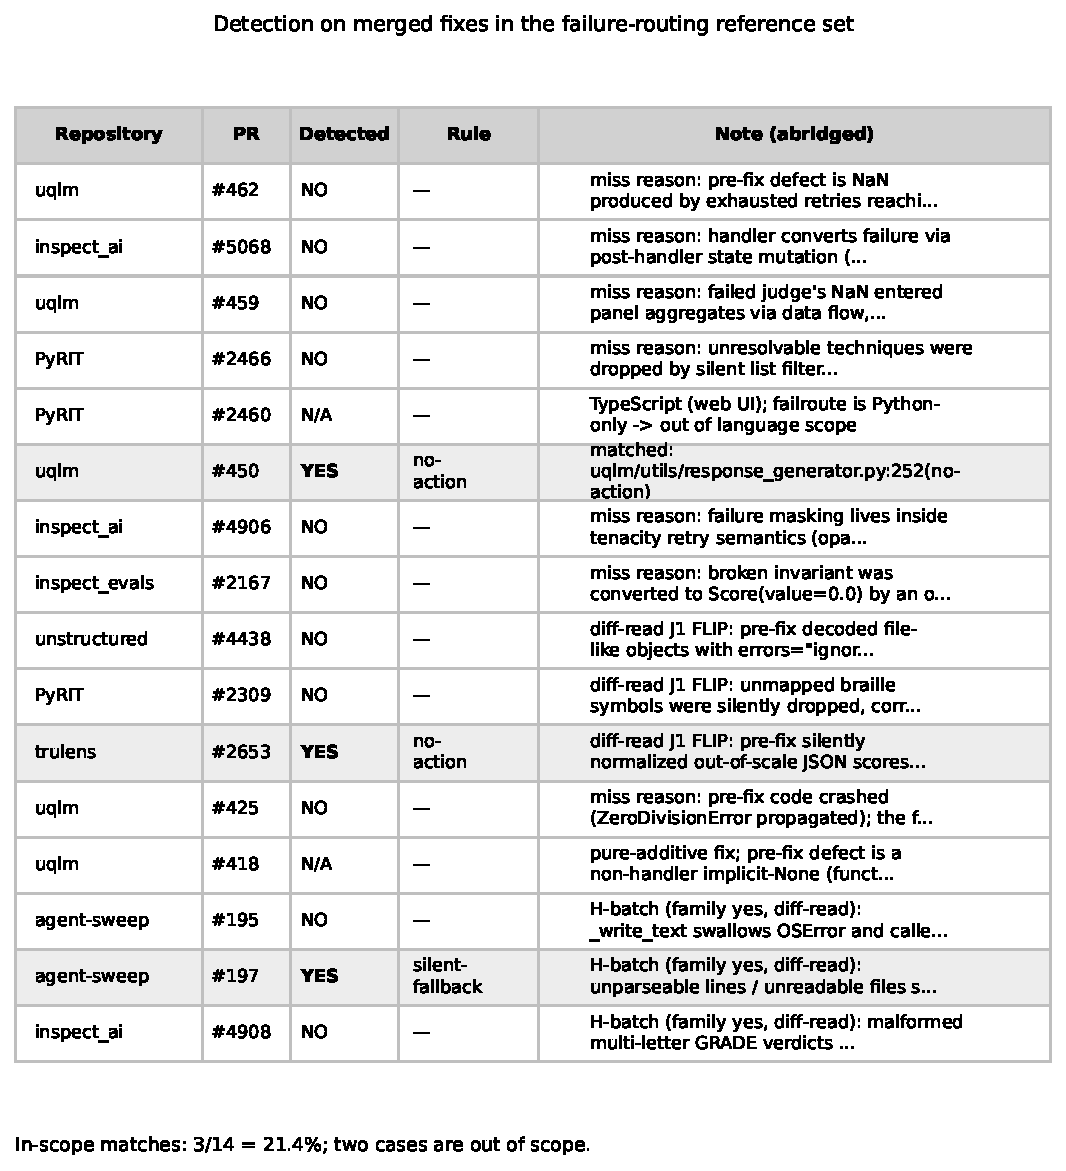
\includegraphics[width=\textwidth]{figures/fig3_reference_matches_by_family.pdf}
\caption{Matches in the curated merged-fix reference set. Shaded rows are
matched; N/A denotes the two out-of-scope cases. Repository and pull-request
identifiers locate each public change. This is not an estimate of population
recall.}
\label{fig:reference-matches}
\end{figure}

\paragraph{Side observation.} In the pre-fix
\texttt{UKGovernmentBEIS/inspect\_ai} \#5068 file the detector flagged
a \emph{different, unfixed} \texttt{silent-fallback} candidate at line 356.
That finding was not adjudicated as a defect in this recall audit.

\subsection{RQ3b --- A tri-source triangulation}
\label{sec:tri}

The original sample contains many CONTRACT and FALSE POSITIVE labels, but
those are LLM judgments rather than independent defect adjudications. The
remaining question is whether maintainer behaviour can distinguish deliberate
contracts from defects that have not been noticed. We compare three evidence
sources that measure different, non-commensurable populations. Table~\ref{tab:arms}
sets out what each source records.

\begin{table}[htbp]
\centering\small
\caption{Three evidence sources and the finite records each describes. The
datasets behind arms 2 and 3 are described below.}
\label{tab:arms}
\begin{tabular}{@{}P{3.2cm}P{3.8cm}P{7.6cm}@{}}
\toprule
Arm & Question & Observed record \\
\midrule
1 --- consequence labels & What did the LLM rounds label in the stratified sample?
& 12/80 (15.0\%) DEFECT labels, all in one package \\
2 --- spontaneous maintainer action & What was changed during the tracked window?
& 13/478 (2.7\%) tracked sites classified FIXED \\
3 --- maintainer response & What happened to the selected family-fix PRs?
& 16/43 (37.2\%) selected PRs merged \\
\bottomrule
\end{tabular}
\end{table}

\paragraph{Records behind arms 2 and 3.}
Arm 2 is a maintainer-behaviour dataset over the same eight
pinned packages, published as \texttt{paper/arm2-tracked-sites.csv}. The
pipeline behind it tracked 2{,}128 \texttt{try} sites across ten releases of
each package and labelled 478 of them FIXED/SURVIVED, discarding 1{,}650
(77.5\%) as too young (924), vanished (681) or mutated (45); none of the 13
FIXED sites traces to a PR submitted from the project account --- the 9
PR-attributed fixes match no PR in that account's record, and the 4 unattributed
ones were cleared by package and content
check. Two properties of that population bound what arm 2 can be compared
against. Its tracking criterion (a handler carrying no raise, log or warn
signal) is weaker than the six rules of Section~\ref{sec:detector}, so only
185 of the 478 rows (38.7\%) carry a \texttt{failroute} rule at the release
where they were first observed. And its package mix is 59.4\% \texttt{deepteam},
against 22.5\% of the 621 findings. Arm 3 is the merged/closed record of family fix PRs submitted from the author's account: the 16 merged members
are itemised in \texttt{paper/merged-pr-recall.csv} --- 8 of them in packages
outside the tracked eight --- and the 27 closed-unmerged members are itemised,
with per-PR closure reasons, in \texttt{paper/h1\_arm3\_classification.csv}
(copied into this artefact set from the unreleased companion repository so the
composition is third-party checkable): 19 self-closed, 1 bot-closed, 3 closed
without reaching the merits, 2 substantively accepted, and 2 adverse on the
merits. Among the 24 PRs not self-closed, 16 merged, seven were maintainer-closed, and
one was bot-closed. One closed PR (\texttt{cvs-health/uqlm}\#427) shares its
substance with merged PR \#462, and two others duplicate separate submissions;
therefore the 43 PRs are not 43 distinct candidate defects. These are descriptive
outcomes in a project-selected set, not an acceptance-rate estimate.

\paragraph{Verdict: directionally consistent, not established.}
The three sources provide different kinds of evidence. The LLM labels describe
consequences in a stratified sample but do not establish defect status. A site
that persists without a recorded fix may be either a contract or an unnoticed
defect. Maintainers accepted many surfaced, project-selected reports, while two
outcomes were adverse on the merits. Their
denominators and selection processes do not define a common estimand. We therefore
report the finite-record counts and leave the defect rate unresolved.

\emph{The arms are not commensurable.} Arm 2's denominator is 478 tracked sites;
arm 3's is 43 defect candidates pre-screened by the author, of whose 16 merged
members 8 lie in packages outside the tracked eight. The counts answer different questions about different populations. The
tracked-site criterion is also weaker than the detector's, so 61.3\% of arm 2's
rows carry no \texttt{failroute} rule at all, while arm 1's labels are attached to
findings. These records cannot support a population-level comparison.

\emph{Why we do not estimate a common rate.} Arm 2 tracks 2{,}128 sites,
but only 478 were classified FIXED or SURVIVED; 1{,}650 were excluded as too
young, vanished or mutated. The records do not establish which tracked sites were
genuine defects, or which excluded sites belong in a risk set. Arm 1's stratified
labels therefore cannot be transferred to arm 2 to estimate defect composition.

\paragraph{No matched sample is available.}
None of the 16 merged family fixes maps to the 478 tracked sites (zero exact file
matches), so the records provide no matched site-level comparison. As context
only, in \texttt{uqlm} none of 12 tracked family sites was classified FIXED,
while all five project-selected family-fix PRs were merged. These are different
sets and the PRs were selected by the project workflow; the counts do not estimate
a common rate.

\emph{What these records support.} Three limited observations.

(i)~The itemised closure record
(\texttt{paper/h1\_arm3\_classification.csv}) shows that maintainer engagement
with surfaced family reports was mostly, but not uniformly, favourable. Of the
24 non-self-closed outcomes, 16 merged, seven were maintainer-closed, and one
was bot-closed. Two additional closures accepted the substance: the gap reported
in \texttt{Giskard-AI/giskard-oss}\#2614 was fixed upstream in a third-party
restatement, and \texttt{cvs-health/uqlm}\#427 was partially re-landed through
merged \#462. Three closures never reached the merits, and two were adverse on
the merits. All outcomes came from a project-selected set.

(ii)~Thirteen of 478 tracked family sites were classified FIXED during the
observation window. Because SURVIVED does not distinguish a contract from an
unnoticed defect, this count cannot establish the underlying defect share.

(iii)~A future study would need maintainer responses to a random sample of
findings to distinguish unnoticed defects from false positives. Such a sample
does not exist in these records and cannot be reconstructed retrospectively.

The three arms describe different units and selection processes. Their counts
cannot be combined into a common defect-rate estimate; the validity limitations
are detailed in Section~\ref{sec:threats}.

\subsection{RQ4 --- Sample review and a detector correction}
\label{sec:rq4}

All four false positives in the sample were \texttt{implicit-fallback}, and all
four had the \emph{same} root cause:
\texttt{\_has\_top\_level\_terminal()} inspected only \emph{direct} statements of
the handler body, so a \texttt{return}/\texttt{raise} nested inside an exhaustive
\texttt{if/else} was invisible. Table~\ref{tab:fpshapes} lists the four real
shapes that triggered it.

\begin{table}[htbp]
\centering\small
\caption{The four shapes that exposed the detector bug.}
\label{tab:fpshapes}
\begin{tabular}{@{}lll@{}}
\toprule
Package & Function & Shape \\
\midrule
deepteam & \texttt{simulate\_baseline\_attacks} & \texttt{if ignore\_errors:
return [...] else: raise} \\
fickling & \texttt{check\_pickle} & nested \texttt{try/except}, every path
returns \\
inspect\_ai & grok \texttt{generate} & \texttt{if/elif/else}, every branch
returns or raises \\
pydantic\_ai & \texttt{execute\_output\_function} & \texttt{if wrap: raise
ToolRetryError else: raise} \\
\bottomrule
\end{tabular}
\end{table}

We implemented a recursive exhaustiveness analysis
(\texttt{\_always\_terminates}) covering \texttt{if/else}, \texttt{with},
\texttt{try/except/finally} and \texttt{match}, added six regression tests derived
from the four real shapes (each failing before the fix), and re-ran the corpus.

\textbf{\texttt{implicit-fallback} findings on the 524{,}229 lines the detector
actually reads: 10 $\rightarrow$ 0.
Total findings: 659 $\rightarrow$ 649 (v0.7.0).} The v0.8.0 precision release
removed 28 more findings through four audited fixes (tuple-typed handlers,
\texttt{warnings.warn} recognised as a signal, \texttt{StopAsyncIteration}
added to the ignore list, conservative optional-dependency probe):
\textbf{649 $\rightarrow$ 621}, with every deletion traceable to a labelled
category or a mechanical criterion --- no labelled DEFECT was removed. The test
suite grew over the same period, from 124 to 130 (the six regression tests of
this subsection) and then to \textbf{158} (twenty-eight more with the v0.8.0
precision release).

The corrected recursive control-flow analysis reduced this rule's ten candidates
in the corpus to zero; the four sampled false positives exposed the shared cause.
More broadly, the stratified labelling pass revealed a detector defect that the unit
fixture corpus did not expose.

\subsection{RQ5 --- What changed under predicate refinement}
\label{sec:rq5}

\paragraph{Provenance and evaluation scope.}
Sections~\ref{sec:detector}--\ref{sec:rq4} use \texttt{failroute} 0.8.0,
pinned by the \texttt{v0.8.0} tag. RQ5 evaluates the released \texttt{failroute}
0.9.1, pinned by \texttt{v0.9.1}; a rescan of the pinned corpus reproduces the
476-finding export in \texttt{bench/rescan-v2/} (verified 2026-09-07). The refactor
was developed against the same corpus and all 140 labels used in this evaluation,
with no held-out set. The results below are therefore descriptive of this
development corpus and do not establish performance on unseen data.

\paragraph{What changed.} v0.8.0's \texttt{silent-fallback} rule asks whether the
handler's body returns or assigns a member of a fixed constant set. That is a
syntactic proxy for the failure-to-value pattern in
Section~\ref{sec:family}; it cannot tell whether the value is an intentional
part of the function's contract. The refactor replaces the constant test with
three further heuristics. \textbf{(1) Value-range membership:}
if the enclosing function's declared return type admits the substituted value,
the tool treats this as possible contract evidence and downgrades the finding ---
applied only to the return channel and only to explicitly declared ranges, never to
an assignment into object state. A type annotation alone neither establishes
intent nor lets the caller distinguish a failed operation from a legitimate
value of the same type. \textbf{(2) Exception--predicate isomorphism:}
whether the handler's work is structurally the same as a \texttt{-> bool} predicate
the codebase already declares. \textbf{(3) Data-flow consequence:} whether the
substituted value escapes the call (returned) or outlives it (assigned to object
state), a proxy for possible caller-visible consequences rather than proof of
them. Every finding now also
carries a severity (INFO, LOW, MEDIUM, HIGH), an isomorphism class, and a static
\texttt{covered\_by} list predicting which lint rules flag this handler. That
list is a table derived by running the four baselines over generated probes rather than
by reading rule names
(\texttt{tools/lint\_mapping\_probe.py} $\rightarrow$
\texttt{bench/lint-rule-mapping.json}). The original shape-based mapping got
three conditions wrong; Result 2 reports the correction and its effect.

\paragraph{Result 1: fewer findings, and more of them already linted.}
Findings fall from 621 to \textbf{476} (617 to 472 distinct handler sites; four
sites are reported twice in \emph{each} frame, because the assign channel emits one
finding per assigned target while the finding identifier is derived from the handler
alone --- an identifier collision in the refactored detector, noted rather than
hidden). The four-linter union's co-location with those findings \textbf{rises}
from 255/621 $=$ 41.1\% to 252/476 $=$ \textbf{52.9\%}; the unmatched count
falls from 366 (58.9\%) to \textbf{224} (47.1\%). These are exact counts in the
pinned corpus under the stated matching rule.

The refactor is not a pruning of the old frame, and treating it as one would
overstate its coherence. Over distinct sites, \textbf{184 disappeared, 39 appeared
and 433 persisted}. Of the 184 dropped sites, 155 (84.2\%) had been
\texttt{failroute}-only; of the 39 added, 15 (38.5\%) were. The losses concentrate
in \texttt{silent-fallback} (177 of 184, plus 4 \texttt{no-action} and 3
\texttt{silent-suppress}); the additions are all \texttt{silent-fallback}.
\texttt{silent-suppress} falls from 19 findings to 16, so RQ1's ``0 of the 19'' is
a property of v0.8.0 and does not carry over to this frame. On these counts, the refinement reduced the candidate list and also reduced
the number of findings not co-located with selected linters. The available label
set cannot establish whether that trade-off improved confirmed-defect detection.

\paragraph{Result 2: exploratory label comparison.}
RQ1 measures candidate-list co-location; RQ2 reports LLM labels for a different
sample. Neither alone establishes which findings are defects. We joined all 140
labels to the refactored frame on (package, file, line) --- the handler's coordinates, deliberately \emph{not} including the rule name,
because the refactor can reclassify a handler without dropping it and one label in the
sample was reclassified from \texttt{implicit-fallback} to \texttt{silent-fallback} ---
104 join and 36 do not; all 36 come from the frozen 80 and are 33
CONTRACT plus 3 FALSE POSITIVE, so \textbf{no observation carrying an LLM DEFECT label was removed}, and only
one of the 36 sits within two lines of a surviving finding --- the failures to join
are deletions, not line drift.

\begin{table}[htbp]
\centering\small
\caption{LLM DEFECT labels by lint co-location among the 104 observations that
join to the refactored frame. The static mapping and empirical co-location agree
on all 104; the label shares describe this clustered, partly purposive set only.}
\label{tab:crosstab}
\begin{tabular}{@{}lrrr@{}}
\toprule
Co-location & LLM DEFECT labels & $n$ & Sample share \\
\midrule
A linter reaches the finding & 12 & 48 & 25.0\% \\
No linter reaches the finding & 1 & 56 & 1.8\% \\
\bottomrule
\end{tabular}
\end{table}

Because the labels are clustered and the 60 supplementary observations were
purposively selected, the table describes this joined set only. It does not
establish a population-level difference or incremental defect yield.

\paragraph{The static \texttt{covered\_by} field was unsound. We measured the whole
mapping and fixed it.}
The inference credited \texttt{bandit:B110} and \texttt{ruff:S110} to every handler
with an inert body, without looking at what the handler catches. Both rules are
broad-only. Before the mapping was measured, the faulty
inference called 87 of 476 findings (18.3\%) novel against co-location's 224 (47.1\%),
and 137 findings it called statically covered were flagged by no linter at all. One of
them is \texttt{garak/analyze/ci\_calculator.py:40}, whose handler is a literal
\texttt{except (ValueError, TypeError): pass}. Running all four baselines on that
single file returns \emph{nothing} --- \texttt{ruff} reports ``All checks passed!'',
\texttt{bandit} and \texttt{flake8} return no rows, \texttt{pylint} scores the file
10.00/10. This is a defect in our own mapping; it made the lint baselines appear to cover
more findings than they actually did and understated failroute's measured novelty.
We report the correction rather than silently changing the comparison.

We did not patch the witness; we measured the mapping.
\texttt{tools/lint\_mapping\_probe.py} generates 68 probes --- eleven caught-type forms
(bare; \texttt{Exception}; \texttt{BaseException}; \texttt{builtins.Exception}; a tuple
of two narrow names; a tuple mixing \texttt{Exception} with a narrow name, with a dotted
name, and with a name no resolver can read; a single narrow name; a dotted narrow name;
and a caught type that is a call expression) crossed with six body forms
(\texttt{pass}, \texttt{...}, \texttt{continue}, a returned constant, an assigned
constant, a discarded comparison), plus both \texttt{contextlib.suppress} forms ---
runs all four baselines over them, attributes every hit to the case whose function span
contains it, and writes the matrix to \texttt{bench/lint-rule-mapping.json}. Every rule
carries a positive control, so a selector that silently matches nothing fails the run
instead of being recorded as ``never fires''. That guard paid for itself twice.
\texttt{ruff} rejects an unknown selector with exit code 2 rather than an empty result
set. And \texttt{pylint} accepts \texttt{W0703} --- the retired id RQ1's baseline
enables --- and reports those messages as \texttt{W0718}: enabling only \texttt{W0703}
emits \texttt{W0718} and nothing else, and over the corpus RQ1's exact selection emits
423 \texttt{W0718}, 134 \texttt{W0702} and 6 \texttt{W0706}, which is the 563 of
Table~\ref{tab:tools}. A reproducer who counts \texttt{W0703} messages finds zero and
would reasonably conclude the broad-except rule never ran.

The measurement found \emph{three} wrong conditions, not the one we started from:
\begin{itemize}[nosep,leftmargin=*]
\item \textbf{Caught type, ruff.} \texttt{S110} and \texttt{S112} fire when the handler
  is bare or catches \texttt{Exception}\,/\allowbreak\,\texttt{BaseException}, including
  inside a tuple of any composition.
\item \textbf{Caught type, bandit.} \texttt{B110} and \texttt{B112} are narrower still:
  bare, or \emph{exactly} \texttt{except Exception:}. They do not fire on
  \texttt{except BaseException:}, on \texttt{except builtins.Exception:}, or on any
  tuple. Gating all four rules on one ``broad'' predicate --- the obvious fix --- would
  have moved the over-credit rather than removed it, and left
  \texttt{pydantic\_ai/\_agent\_graph.py:205}, an
  \texttt{except BaseException: pass}, wrongly credited.
\item \textbf{Body form.} \texttt{S110} and \texttt{B110} are literally
  ``try-except-\emph{pass}'': they fire on a body of \texttt{pass} and not on a body of
  \texttt{...}, even for a bare handler. This detector's own notion of an inert body
  accepts both forms, so the distinction had to be made in the mapping rather than
  inherited from that flag. On this corpus that third condition changes no number ---
  all 146 over-credited findings have a \texttt{pass} body --- but it is a real defect
  and the probe pins it.
\end{itemize}

Correcting the caught-type conditions then exposed an error in the \emph{opposite}
direction, which is the argument for measuring rather than patching. The predicate
deciding whether a handler catches \texttt{Exception} gave up entirely when any member
of a caught tuple was not statically resolvable, so
\texttt{except (anyio.get\_cancelled\_exc\_class(), Exception):} --- three instances in
\texttt{inspect\_ai} --- was classified as narrow and kept only its body-form credit
(\texttt{bandit:B110}, \texttt{ruff:S110}), losing the two caught-type credits that
do fire on it (\texttt{pylint:W0718}, \texttt{ruff:BLE001}); and \texttt{bandit:B110}
should not have been there either, since B110 fires on no tuple at all. That error
over-states novelty. Leaving it in place would have made the corrected figure look
better for the tool than the truth.

The correction is held by 36 tests, and a suite that passes proves nothing about
itself, so \texttt{tools/refix\_replay.py} rebuilds the pre-correction predicate
in a scratch tree and runs the same 36 against it: \textbf{21 fail}. Red before
the change and green after it, on identical tests --- the suite constrains the
mapping rather than accompanying it.

\textbf{Before and after.} The correction removes credit from \textbf{146} findings and
adds it to 3. Of the 146, \textbf{137} become statically novel and 9 stay covered
because a rule that genuinely fires on them is still credited. All 146 are
\texttt{no-action} findings --- 93 at INFO, 48 at MEDIUM and \textbf{5 at HIGH}.
Statically novel findings go from 87 (18.3\%) to \textbf{224 (47.1\%)}, and HIGH
findings with no lint coverage from 20 to \textbf{25}. What the detector \emph{reports}
does not change at all --- 476 findings before and after --- and neither do the
empirical co-location figures (252 covered, 224 novel), because those come from running
the linters rather than from inferring anything about them. That the statically novel
count and the empirically novel one are now the same number is not a coincidence; see
the next paragraph.
\texttt{tools/rq5\_refactor\_delta.py} recomputes the whole comparison from the
preserved pre-fix export; \texttt{tools/lint\_mapping\_probe.py --check-parity}
re-derives the mapping and fails if the shipped inference drifts from it; and 36 tests
pin the same conditions, including the reverse direction (a narrow handler must lose the
credit, and widening it to bare must restore it).

\paragraph{A residual we had not eliminated --- and then did.}
Five findings of the 476 disagreed with the empirical measure. All five are
\texttt{except Exception:} handlers that return or assign a constant; the corrected
inference credits \texttt{pylint:W0718} and \texttt{ruff:BLE001}, \texttt{BLE001}
does fire at exactly that line, and yet the co-location run recorded no linter there
at all. Three explanations were tested and ruled out: it is not a parse failure
(\texttt{pylint} rates \texttt{model/\_providers/openai.py} 9.96/10 with no fatal or
syntax message, and the file's single \texttt{except Exception} is the one it
declines to flag); it is not an inline pragma (none of the four files contains the
string ``pylint''); and it is not the \texttt{as} binding, which real code uses and
the probe originally did not --- tested directly, \texttt{W0718} fires on
\texttt{except Exception:}, on \texttt{except Exception as e:} and on the same
handler that uses \texttt{e}, and does not fire on a bare \texttt{except:}. The
synthetic case that matches these five \emph{does} earn \texttt{W0718} in the probe,
so the discriminating condition was something about their context. It was our
harness, not the linter: all four files sit under a directory with no
\texttt{\_\_init\_\_.py}, and the directory-based invocation of \texttt{pylint} described in
Section~\ref{sec:rq1} did not analyse them. Handed the files
directly, \texttt{pylint} emits \texttt{W0718} at the disputed line in every one of
the five. Two corrections follow. First, with the harness fixed, the static
\texttt{covered\_by} mapping and empirical co-location agree on all 476 findings:
224 are novel by both criteria. Second, this reverses the direction of the residual
bias. \texttt{W0718} is in RQ1's selected \texttt{pylint} rules and fires on all
five disputed handlers, so the directory-based run under-counted linter coverage
and overstated novelty by five findings (229 before correction, 224 after). None
of the five was labelled, so the 12-of-48 versus 1-of-56 crosstab is unchanged.

The corrected static mapping agrees with empirical co-location on all 476
findings. The mapping repair changed coverage classifications but did not change
the LLM-label join: none of the five disputed handlers carried an original
DEFECT label. Among the original labels, no narrow-typed handler carried that
label; one of 23 purposively selected supplementary labels on narrow-typed
handlers did. This contrast does not support generalization.

\paragraph{Result 3: contribution of the isomorphism layer.} Of the 476 findings the
isomorphism layer classified \textbf{none} as isomorphic: 254 non-isomorphic, 206
unknown, and 16 with no class at all (the \texttt{silent-suppress} findings, which
have no handler). A layer that never produces a positive classification contributed
nothing to the separation measured above; whatever the refactor achieved came from
layer 1 (declared value ranges) and layer 3 (escape channel). Severities across the
frame: 208 HIGH, 126 MEDIUM, 129 INFO, 13 LOW.

\paragraph{Result 4: what the refactor did accomplish.} All 13 observations
carrying LLM DEFECT labels survive it, and all 13 receive HIGH severity; this
describes label disposition, not confirmed defects. Of the 122
CONTRACT labels, 33 were dropped and 25 reduced to INFO or LOW: 58 of 122, 47.5\%.
Restricting to the case layer 1 was built for, contracts whose enclosing function
\emph{declares} a None-admitting return type, 35 of 38 (92.1\%) were dropped or
reduced; for a literal \texttt{-> None}, 22 of 23 (95.7\%). Not all of them, and the
exceptions are the interesting part: three declared-contract findings still report
at HIGH or MEDIUM, and \textbf{two} labelled FALSE POSITIVES survive at HIGH. One is
\texttt{pydantic\_ai/ui/\_event\_stream.py:293}, an async generator whose handler
propagates the error elaborately and which the refactor reports \emph{twice}. The
other is \texttt{fickling/polyglot.py:150}, which the frozen sample labelled as an
\texttt{implicit-fallback} over-call and the refactor now reports as
\texttt{silent-fallback} instead, still at HIGH. The second one is visible only
because the join in Result 2 keys on the handler's coordinates and not on the rule
name: a rule-inclusive join counts a reclassified handler as a deletion and quietly
reports one surviving false positive instead of two. And 55
of the 122 CONTRACT labels sit in functions with no declared return annotation at
all, so layer 1 cannot apply to them by construction. That is the ceiling on how
much noise this design can remove: without type information, the declared-contract
test has nothing to read.

\paragraph{The 60 supplementary labels.} RQ2's 80 labels were drawn from the
v0.7.0 frame; 72 survive into v0.8.0 and fewer into this one, which is too small a
base for a crosstab. We labelled 60 further findings, written to
\texttt{paper/annotations-v2-additions.csv} --- a new file. The frozen
\texttt{annotations.csv} and \texttt{annotations-second-pass.csv} are unchanged and
remain SHA-locked; nothing in RQ2 was re-labelled to suit this section. Method:
candidates were drawn from the refactored frame with priority on sites whose status
the refactor changed and on sites no linter reaches; each was labelled by reading
the pinned corpus source, and the detector's own severity, isomorphism and
\texttt{covered\_by} values were recorded into the row \emph{after} the rationale was
written, so the rationale is not a restatement of the verdict; every row carries its
rationale, the enclosing signature, and a flag for whether the site is new in this
frame. One row is marked in its own rationale as the weakest of the 60 --- a
borderline CONTRACT that a second annotator could reasonably call DEFECT --- rather
than being quietly resolved. The outcome was 1 DEFECT, 58 CONTRACT, 1 FALSE
POSITIVE. Labels were written by an LLM agent, the same process as RQ2's, and
inherit every limitation RQ2 states about it, including that agreement between runs
of one model family is compatible with shared bias, not proof of accuracy; we did not run the 60
twice. The 60 are \emph{not} a random sample, so the 140-label figures support a
within-sample description only, not a wider inference.

\paragraph{The one DEFECT label in the novel remainder.} The single DEFECT
label among the 56 non-co-located observations is
\texttt{garak/probes/dan.py:134}, a narrow-typed handler from the supplementary
round. It is one LLM label from a purposively selected sample, not an independently
confirmed finding or an estimate of defect share. It shows only that the observed
novel cell was not empty of DEFECT labels.

\paragraph{Reproducing this subsection.}
\begin{verbatim}
.venv/bin/python tools/rescan_corpus.py --out bench/rescan-v2 --with-context
.venv/bin/python tools/coverage_union.py --findings-dir bench/rescan-v2 \
    --out bench/corpus-coverage-union-v2.json \
    --emit-per-finding bench/corpus-coverage-per-finding-v2.jsonl
.venv/bin/python tools/coverage_union.py --findings-dir bench/rescan-f2 \
    --out bench/corpus-coverage-union-621frame.json \
    --emit-per-finding bench/corpus-coverage-per-finding-621.jsonl
.venv/bin/python tools/e722_baseline.py        # -> bench/e722-baseline.json
.venv/bin/python tools/rq5_refactor_delta.py   # -> bench/rq5-refactor-delta.json
PYTHONPATH=src .venv/bin/python tools/lint_mapping_probe.py --check-parity
    # -> bench/lint-rule-mapping.json; re-runs all four baselines over 68
    # generated probes and exits non-zero if the shipped covered_by table
    # drifts from what those baselines actually do
.venv/bin/python tools/pinned_rescan.py --out /tmp/pinned-v080
    # -> re-scans the pinned corpus with the v0.8.0 detector, from a git
    # worktree at that tag, using that tree's own src and exporter; prints
    # PINNED_TOTAL=621 plus the per-rule and per-package counts. This is what
    # the claims asserting v0.8.0's historical scan results now run through.
PYTHONPATH=src .venv/bin/python tools/refix_replay.py
    # -> rebuilds the pre-correction covered_by_for in a scratch tree and runs
    # the 36 mapping tests against it; prints REFIX_REPLAY 21 failed, 15
    # passed. The fail-to-pass half of the correction's evidence.
\end{verbatim}
The checked-in exports make both frames reproducible without overwriting the
frozen v0.7.0 scan: \texttt{bench/rescan-f2/} contains the 621-finding v0.8.0
frame, and \texttt{bench/rescan-v2/} contains the 476-finding refactored frame.
Running the corresponding \texttt{coverage\_union.py} commands reproduces the
reported per-rule and per-tool counts.

\subsection{Control-corpus comparison}
\label{sec:control}

\paragraph{Design.} The main corpus is dominated by one handler shape: 134 bare
\texttt{except:} clauses, 131 of them in a single package, holding all 12 original DEFECT-labelled sites. Any claim of the form ``the lint baseline already covers the defects''
may therefore be an artefact of code style rather than a general fact. The control
corpus inverts the style: across its eight package bodies (263 \texttt{.py} files,
109{,}400 lines, 842 handlers) there is exactly one bare \texttt{except}, in
\texttt{msgpack/fallback.py:812}, whose handler resets the buffer and re-raises
--- so even the single E722 candidate is a non-defect. The detector build is the
frozen 0.9.x predicate, unmodified; the four baselines run with RQ1's exact rule
selection and $\pm$1-line matching. The four first packages contribute 243 handlers
and 0 bare clauses; the four added for domain diversity contribute 599 handlers
and the 1 re-raising bare clause.

\paragraph{Result: the trivial baseline behaves differently across these
corpora.} Table~\ref{tab:control} contrasts the selected packages. Finding
density is 21.0\% (476/2{,}270) in the main corpus, 15.6\% (38/243) in the
four-package control core, and 18.3\% (154/842) across all eight control
packages. These are descriptive densities in purposively selected corpora, not
estimates for broader classes of software. \texttt{flake8 --select E722}
returns 134 candidates on the main corpus, including all 12 original
DEFECT-labelled sites; on the control corpus it returns one candidate, which is
a re-raise and carries no DEFECT label.

\paragraph{Result: no misses were adjudicated in the read set.} Of the control
corpus's 243 handlers the tool reports 38; 114 unreported handlers contain a
\texttt{raise} and need no review; the remaining 91 silent-and-unreported
handlers were each read. None was adjudicated a miss under the stated protocol:
the cases were optional-import and capability probes, \texttt{StopIteration}
protocol handling, \texttt{dict.get} and \texttt{list.index} sentinels,
documented best-effort fallbacks (\texttt{requote\_uri},
\texttt{get\_unicode\_from\_response}), data-model protocol returns
(\texttt{NotImplemented}), and CLI exit paths. This is an exhaustive review of
that finite read set by one annotator, not proof of zero misses in related code.

\paragraph{The four diversity packages agree.} \texttt{click} (31 findings, 13
HIGH), \texttt{anyio} (45 findings, 1 HIGH), \texttt{pydantic} (40 findings, 1
HIGH) and \texttt{msgpack} (0 findings) reproduce the pattern: 12 of the 15 HIGH
findings are \texttt{except Exception} capability probes already covered by
\texttt{BLE001}/\texttt{W0718} (Windows-console shims, stream predicates,
\texttt{TaskGroup} propagation with explicit re-raise paths). The 3 uncovered
HIGH findings are contracts on reading: \texttt{click/core.py:161} is a
\texttt{list.index} probe returning infinity as the documented sort key;
\texttt{click/types.py:269} converts the user's \texttt{ValueError} via
\texttt{self.fail}, which raises \texttt{UsageError} --- the exception escapes
through a call rather than a \texttt{raise} statement, a shape no callee-local
rule can see; \texttt{pydantic/v1/\_hypothesis\_plugin.py:125} is a
\texttt{contextlib.suppress(Exception)} digit search in hypothesis test-support
code, confirming the SIM105-adjacent blind spot of Section~\ref{sec:rq1} from the
other side.

\paragraph{A fourth intra-procedural undecidability instance.}
\texttt{connectionpool.py:812} names a new false-positive mechanism:
\textbf{state-flag amplification}. The finding is \texttt{clean\_exit = False} (set
alongside \texttt{release\_this\_conn = False}), a control-flow flag consumed in
\texttt{finally} and after the handler; the \texttt{amplifies} criterion (``the
value outlives the call'') promotes it to HIGH exactly as it would a substituted
return value. Telling the two apart requires knowing where the variable is
consumed, which lies outside the handler. Like the three constructed
counterexamples and the \texttt{exception\_escapes} case below, it is documented
here and left in the code: each is an instance of the limit the paper argues,
and patching them would weaken the evidence they constitute.

\begin{table}[htbp]
\centering\small
\caption{Style-opposite corpora, same detector build and baseline selection.
Densities are findings per handler inside the scan roots. The E722 row reports
coverage of the original 80-item LLM-labelled sample only; one supplementary
LLM DEFECT label lies outside E722. Control-corpus readings were made by one
annotator and are not the same label process as Group~A.}
\label{tab:control}
\begin{tabular}{@{}lrrr@{}}
\toprule
 & Group~A & B core (4 pkgs) & B all (8 pkgs) \\
\midrule
Handlers & 2{,}270 & 243 & 842 \\
Bare \texttt{except:} & 134 & 0 & 1 (re-raise) \\
Findings & 476 (21.0\%) & 38 (15.6\%) & 154 (18.3\%) \\
HIGH & 208 & 6 & 21 \\
Unique HIGH (\texttt{covered\_by} empty) & 25 & 2 & 5 \\
E722 candidates & 134 & 0 & 1 \\
E722 coverage of original 80-sample labels & 12/12 & --- & --- \\
Recorded DEFECT labels & 12/80 + 1/60 & 0 of 38 & 0 of 38, 0 of 15 new HIGH \\
\bottomrule
\end{tabular}
\end{table}

\paragraph{Reproducing this subsection.}
\begin{verbatim}
PYTHONPATH=src .venv/bin/python tools/control_rescan.py --check
    # -> verifies bench/control-rescan/<pkg>.jsonl against a fresh fetch
    # (SHA-256 checked per paper/corpus-lock-control.json) and re-scan;
    # prints CHECK-OK per package, exits non-zero on any drift.
\end{verbatim}

\section{Discussion}

\paragraph{The detector is a review queue, not an alarm.}
On these pinned trees, \texttt{flake8 --select E722} returns 134 candidates and
contains all twelve DEFECT-labelled sites in the original sample of 80. This is a
shorter candidate list containing all twelve labels from the original sample, not
proof that E722 captures all confirmed defects. The supplementary sample adds one DEFECT label outside
E722, but it comes from the same LLM process and is not an independently confirmed
increment. The records do not establish a true defect yield for either detector.
They do support a practical evaluation rule: compare against simple lint
baselines, report the rule selection, and require independent adjudication before
calling findings defects. One original sample label describes a fail-open security
verdict in a red-teaming tool; that case illustrates why the construct merits
study, not that this detector has measured its prevalence.

\paragraph{The triangulation identifies a limit of the validation design.}
The label share, cluster share, observed maintainer fixes and project-selected PR
outcomes describe different units and selected records. None identifies the defect
composition of the tracked sites or a common denominator across arms. The evidence
therefore supports separate descriptive observations, not a shared defect rate.
A future study would need independent contract adjudication and maintainer
responses to a random sample of findings.

\paragraph{Labels cluster by package.}
In the original sample, all twelve DEFECT labels occur in one package and three
copied families; the other seven packages have none. This association does not
establish a causal effect of codebase maturity or rule design. It supports
reporting package-level composition in future samples, rather than treating every
finding as an independent bug.

\paragraph{Four layers of overfitting, stated against ourselves.}
The refactor was assessed against data available during its development; it is
in-sample engineering evidence, not out-of-sample validation. First, the acceptance gates demand no-regression on the same
corpus the patches were developed against, so every patch is fitted to its own
test set by construction. Second, all 140 labels (80 + 60) were available
during development; there is no held-out set, and the 60 supplementary labels
were drawn precisely from sites whose status the refactor changed. Third, several
counterexamples that changed the interpretation --- the constructed probes below,
the state-flag mechanism of Section~\ref{sec:control}, and the mapping defects of
Section~\ref{sec:rq5} --- were identified during subsequent review of this project. Fourth: callee-local analysis cannot
define ``the caller cannot distinguish'' without caller intent, so its
separation criterion is necessarily a syntactic proxy, and proxies fitted on one
style fail on the next. In the selected control corpus, the single annotator
assigned no DEFECT label to any of the 38 core findings; this does not establish
that the detector has no unique contribution on other code.

\paragraph{The limits of caller context.}
Under the study's definition, whether a handler violates a contract can depend on
what its caller expects. This paper does not build a call graph or recover caller
intent, so it does not establish whether caller context would resolve any
particular finding. A future evaluation should compare a reproducible
interprocedural analysis against independent contract adjudication.

\paragraph{Constructed probes of the predicate boundary.}
Three minimal probes were checked against the frozen 0.9.1 build on 2026-09-06:
(1) a boolean predicate returning \texttt{False} on a database timeout is missed
when its handler catches a specific exception; (2) an \texttt{Optional}-returning
function returning \texttt{None} on a Redis error is likewise missed; and (3) a
validation loop with the \texttt{try} outside the loop and a \texttt{return
False} handler is reported at HIGH. The first two expose possible false negatives;
the third exposes a possible false positive. Together with the
\texttt{exception\_escapes} case and state-flag amplification, they document
limits of the evaluated intra-procedural predicate. They were not changed in this
study.

\paragraph{The \texttt{contextlib.suppress} blind spot is real.}
0/19 of the findings are visible to the four selected rule sets, and none is
reported by \texttt{ruff} with all 969 of its rules enabled or by \texttt{pylint}
with its full default message set either. Ruff's SIM105 rule recommends
a refactoring to \texttt{contextlib.suppress}; our supplementary semgrep rule
co-locates with 18 of the 19 findings.

\section{Threats to validity}
\label{sec:threats}

The first five items are the limitations on which the triangulation verdict in
Section~\ref{sec:tri} depends; the rest are the study's other threats.

\begin{itemize}[nosep,leftmargin=*]
\item \textbf{Limitation 1 --- the labelling arm is LLM-judged.} Both labelling
  rounds were performed by LLM agents, not human raters; the rounds agreed on
  80/80 items. Agreement between these automated runs does not establish
  independent adjudication or label accuracy and is compatible with shared
  model bias.
  All arm-1 proportions inherit this limit. The committed
  artefacts record the labels and the rationales but not the model identity or
  version, so a third party cannot re-run the labelling bit for bit. We were not
  able to recover that identity and therefore do not name a model: every DEFECT
  proportion in this paper is an LLM label share under an unrecoverable model
  configuration, and the weighted projection inherits exactly that limitation.
\item \textbf{Limitation 2 --- SURVIVED is ambiguous in this family.} In the
  maintainer-behaviour dataset, SURVIVED can only be read as ``nobody acted'';
  it can \emph{not} be read as ``maintainers consider it a deliberate
  contract'', because for silent defects the two are observationally identical.
  Any number derived from arm 2 inherits this reading restriction.
\item \textbf{Limitation 3 --- arm-3 selection and unit.} The 43 reports were
  selected through the project workflow and include 19 self-closures, one bot
  closure, 16 merges, and seven maintainer closures. Thus 16/43 is the merge
  share of project-selected PR records, not a maintainer-acceptance rate. The
  record is frozen at 2026-09-01; two submissions duplicate other submissions,
  one shares substance with a counted merge, and 8 of the 16 merged fixes lie
  outside the tracked packages. A merge records acceptance of a code change,
  not independent confirmation of a defect or representativeness.
\item \textbf{Limitation 4 --- the triangulation's arms are not
  commensurable.} Arm 1 counts labelled findings, arm 2 counts tracked sites, arm 3
  counts project-selected pull requests, and 8 of arm 3's 16 merged cases
  lie outside the tracked packages. The records therefore do not support a shared population-level rate; we report
  only their separate finite-set observations.
\item \textbf{Limitation 5 --- arm 2's denominator is a convention, and its
  population is not the detector's.} The pipeline tracked 2{,}128 sites and labelled
  478 of them, discarding 1{,}650 (77.5\%) as too young (924), vanished (681) or
  mutated (45); nothing in the data selects among the resulting risk sets. Its tracking criterion --- a handler carrying no raise, log
  or warn signal --- omits the detector's three exemption gates and its
  fallback-value analysis, and never considers \texttt{contextlib.suppress} at all,
  so only 185 of the 478 rows (38.7\%) carry a \texttt{failroute} rule. Arm 1's
  defect share is measured on findings and does not transfer to that
  population.
\item \textbf{Sample size.} $n=80$ of the v0.7.0 frame (659). Per-rule and
  per-package cells are small (\texttt{masked-exception} $n=1$); proportions
  describe the sample and should not be read as population rates.
\item \textbf{Sample frame changed under the sample.} The draw came from
  v0.7.0's 659; 72/80 coordinates survive in v0.8.0's 621, and the deletions
  removed zero labelled DEFECTs --- but the surviving 72 are no longer a random
  sample of the current frame. Label proportions are stated for the v0.7.0
  frame only.
\item \textbf{Package selection is not random.} The eight packages were chosen
  because the author had prior contribution history in them. \texttt{deepteam} in
  particular is a package where a candidate defect family had already been
  reported from the author's account. This prior selection may inflate the
  overall DEFECT-label share. The seven-package 0/66 figure gives the comparison
  without that package.
\item \textbf{Curated reference set shares the project's submission pipeline.}
  The 16 merged family fixes were submitted from the author's account as part of a
  project that used AI-assisted software development; per-PR divisions of work are
  not documented. A maintainer merge
  records that the change was acceptable to the project --- it is not a
  maintainer finding that the pre-fix behaviour was a defect, and it says
  nothing about representativeness.
  The family adjudication of all 75 merged PRs was done by reading diffs (52
  earlier title-only judgements were re-verified from diffs in a dedicated
  pass, with 3 corrections).
\item \textbf{Co-location $\neq$ equivalent detection}
  (Section~\ref{sec:rq1} caveat). A nearby warning may concern a different
  property, while a warning farther than one line away may still be relevant.
  The reported co-location count is neither a measured semantic coverage rate
  nor a strict bound on one.
\item \textbf{The fifth baseline tool is ours.} The semgrep rule counted in the
  five-tool union was developed within this project; coverage attributed to it is
  self-supplied.
\item \textbf{Construct validity (Section~\ref{sec:rq3}).} The detector
  operationalises local handlers and \texttt{contextlib.\allowbreak suppress}; 64.3\% of
  fixes in the curated reference set lie outside those shapes. The corpus
  counts and reference-set recall are scoped to the pinned records.
\item \textbf{Control scope is two styles, not the ecosystem.}
  The control comparison covers a zero-bare-\texttt{except} infrastructure style
  against the main AI/ML style; both are Python, both are PyPI. The conclusion
  carried by Section~\ref{sec:control} is scoped to those two corpora, this
  detector build, and this adjudication protocol. A third style, another
  detector, or another annotator could move it, and the finite read-set labels do not estimate defect prevalence in disciplined code.
\item \textbf{Control adjudication is single-annotator.} The 38 findings and
  the 91 recall-side handlers were read once, by one annotator, with history,
  issue-record and test evidence taken only for the 2 unique HIGH findings;
  the remaining 36 + 91 rest on in-source contract evidence (docstrings,
  guarded read sites, explicit fallback comments, re-raise paths). Borderline
  CONTRACT-vs-DEFECT calls were resolved toward CONTRACT wherever a documented
  policy existed; the direction of that bias is stated so a re-adjudication
  can test it. These readings do not establish independent human adjudication.
\item \textbf{Known predicate limits remain in the shipped version.}
  The three constructed probes, the state-flag amplification
  (Section~\ref{sec:control}) and the \texttt{exception\_escapes} case
  (Section~\ref{sec:rq5}) document false-negative and false-positive modes of
  the 0.9.1 predicate. They are examples of its limits, not an exhaustive list.
\item \textbf{Five DEFECT labels have an unestablished mechanism.}
  In five labelled sites, the \texttt{try} body contains the discarded comparison
  \texttt{self.score == 1}; tested values did not raise, but attribute access or
  overloaded equality can raise or have side effects for other objects.
  \texttt{silent-fallback} flags the handler's assignment shape without showing
  that this comparison converts a failure into a wrong caller-visible value.
  The frozen LLM labels remain DEFECT, but these five cases are not confirmed
  instances of the stated failure-conversion mechanism. The function
  \texttt{is\_successful} has no caller in the pinned source distribution, and
  the initial value of \texttt{self.success} depends on an external
  \texttt{BaseMetric} implementation unavailable in the reproduction
  environment. The runtime path therefore remains unverified. The labels were
  not re-adjudicated; this limitation changes their interpretation, not the
  frozen annotation record.
\item \textbf{Version pinning is a snapshot.} All findings are relative to the
  pinned versions in \texttt{paper/\allowbreak corpus-lock.json};\allowbreak{} upstream may have fixed or
  introduced instances since.
\end{itemize}

\section{Related work}
\label{sec:related}

\paragraph{Failure handling as an empirical object.}
Exception handling has a long empirical literature in statically typed languages:
Cabral and Marques' field study of Java and .NET~\cite{cabral2007} documented how
often exceptions are caught and swallowed; Sawadpong et
al.~\cite{sawadpong2012} characterised exception-handling \emph{defects}; and de
P\'adua and Shang quantified the prevalence of named exception-handling
anti-patterns over a large corpus~\cite{depadua2017prevalence} and revisited
developer practice through exception-flow analysis~\cite{depadua2017flow}. That
line of work asks \emph{whether} anti-patterns occur and \emph{how often}, and it
is our closest neighbour: we inherit its premise that handling shape is
measurable, and change the question. On a corpus of Python AI/ML packages, the
same syntactic shapes can receive different readings in context. In our
80-item sample, 64 observations received a CONTRACT label, 12 a DEFECT label,
and 4 a FALSE POSITIVE label from LLM agents. These are judgments from one
labeling process, not confirmed contracts or defects, and the sample does not
estimate their prevalence. The present study makes that uncertainty explicit
rather than treating shape counts as defect counts.

\paragraph{Why generic rules get muted.}
A second body of work explains the reception of such numbers. Developers report
false positives and noise among the reasons they ignore or abandon static
analysis~\cite{johnson2013}; Ruthruff et al.\ made \emph{actionability} an
experimental target rather than a slogan~\cite{ruthruff2008}; Google's Tricorder
and FindBugs-Fixit programmes illustrate the value of filtering, prioritisation
and a suppression path in deployed analysis
tools~\cite{sadowski2015,ayewah2010,sadowski2018}. User-centred and follow-up
studies reach the same ordering from the other side: what developers need is a
warning they can act on~\cite{do2022,yedida2023}, and the mitigation of false
positives remains an open problem rather than a solved one~\cite{guo2023}.
WarningsGuru operationalised relevance with statistical bug
models~\cite{querel2018}, and Hu et al.\ recently measured the other end of the
same pipe --- which warnings developers actually suppress, and on what
grounds~\cite{hu2025suppressed}. Crisan and McNutt frame linting as a
sociotechnical activity~\cite{crisan2025}. Our case study examines why some
syntactic matches may reflect intentional fallback contracts, and where local
code shape alone cannot settle that question. The available labels do not
establish the relative actionability of this detector and its baselines.

\paragraph{Silent failure in machine-learning systems.}
The systems literature supplies the stakes. Sculley et al.\ named the pipeline
coupling and glue-code debt that makes ML behaviour brittle~\cite{sculley2015};
Polyzotis et al.\ proposed continuous data validation as the corrective at the
data boundary~\cite{polyzotis2019}; the ML Test Score encoded a rubric that tests
the pipeline rather than the model alone~\cite{breck2017}; Amershi et al.\ and
Paleyes et al.\ documented challenges during integration and deployment as
well as model development~\cite{amershi2019,paleyes2022}; Sambasivan et al.\ traced how a data
problem cascades through a high-stakes system until it surfaces as an unexplained
outcome~\cite{sambasivan2021}; and Dixit reported silent data corruption at scale
in production hardware, where no exception is raised at all~\cite{dixit2023}.
Zhang et al.\ position testing and robustness techniques across that same
spectrum~\cite{zhang2022}.

\paragraph{How this study differs from the cited work.}
The studies by de P\'adua and Shang~\cite{depadua2017prevalence} and Hu et
al.~\cite{hu2025suppressed} examine, respectively, the frequency of handling
shapes and developers' responses to warnings. This paper adds a limited case
study of LLM labels for sampled Python AI/ML findings and of co-location with
selected syntactic lint rules: 12 of 80 sampled findings carry DEFECT labels,
concentrated in one package, while four selected lint-rule sets co-locate with
255 of 621 candidates. The added evidence is descriptive and does not confirm
the labels or estimate prevalence.

\section{Conclusion}

Across eight pinned AI/ML Python packages, the v0.8.0 detector reported 621
local exception-handling candidates in 524{,}229 scanned lines. Four selected syntactic
linter rule sets were not co-located with 366 candidates under a $\pm$1-line
criterion. This is a finite-corpus comparison; co-location does not establish
equivalent detection, and the candidates are not confirmed defects.

In the original 80-finding sample, LLM agents assigned 12 DEFECT, 64 CONTRACT,
and 4 FALSE POSITIVE labels. The DEFECT labels cluster in three repeated code
families in one package, and five of the twelve have an unestablished
failure-conversion mechanism. The labels are not independent adjudications.
Against the curated merged-fix reference set, the detector matches three of 14
in-scope cases; nine route failure outside an except-handler. This set does not
estimate recall over the software ecosystem.

The refined predicate reduced the candidate count to 476 and increased
four-linter co-location from 41.1\% to 52.9\%. Among 140 LLM-labelled
observations, 104 joined the refined frame; 12 of 48 co-located and 1 of 56
non-co-located observations carried DEFECT labels. The additional 60 observations
were selected purposively, labels are clustered, and the refactor was developed
against the same corpus and labels. The comparison is descriptive and does not
establish incremental defect yield.

The simple \texttt{flake8 --select E722} rule produced 134 candidates and
included all twelve original DEFECT-labelled sites. This is equal coverage of
the twelve labels in a shorter candidate list, not evidence of equal coverage of
confirmed defects or of E722's precision. The practical implication is to treat
static-analysis output as a review queue, compare against simple baselines, and
require independent adjudication before calling a candidate a defect. A stronger
validation study would use independent contract adjudication, held-out packages,
and a sampling design that draws from both detector and baseline findings.

\section{Reproduction and artefacts}
\label{sec:repro}

The empirical counts and comparisons are generated from scripts in
\texttt{tools/} against the pinned corpus in \texttt{paper/corpus-lock.json};
manual adjudications are recorded in the accompanying ledgers. All paths below are
relative to the root of the public repository
\url{https://github.com/feiiiiii5/failroute} (MIT licence); the detector itself is
released as \texttt{failroute} on PyPI,
\url{https://pypi.org/project/failroute/}. RQ1--RQ4 analyze \texttt{failroute} 0.8.0; RQ5 analyzes 0.9.1. The pinned
commit \texttt{3b4c567} contains the underlying datasets, exports and scripts
for the reported numerical results, including the post-release ledgers and
corrected baseline invocation. The figure PDFs in this submission have later
layout edits but unchanged plotted counts; they are included in the arXiv
source package. The v0.8.0 release tag
alone does not reproduce every table. The committed \texttt{bench/rescan-f2/}
export records the 621-finding frame; \texttt{bench/rescan-v2/} records the
476-finding refactored frame (freshly reproduced 2026-09-07).

The pinned 0.8.0 suite contains 158 tests; the 0.9.1 release contains 221 tests.
All 15 release test jobs across Ubuntu, macOS and Windows and Python 3.9--3.13
passed, along with the quality job. The 0.8.0 unit corpus v6 has 36 positive and
32 negative fixtures. For 0.9.1, the revised 34/34 fixture set is labelled v7;
five narrow-type \texttt{contextlib.suppress} cases changed to negative and three
other cases changed in the opposite direction. Every corpus scan reported here was
run on macOS arm64; the CI matrix exercises tests, not scans.

\begin{verbatim}
git clone https://github.com/feiiiiii5/failroute && cd failroute
git checkout 3b4c567                # pinned commit: every artefact the tables use
python -m venv .venv && . .venv/bin/activate
pip install '.[test,paper]'   # pytest + matplotlib + 4 linters + bugbear
python tools/fetch_corpus.py         # pinned sdists -> paper/corpus/
    # version+sha256 pinned in paper/corpus-manifest.json; fetch verifies each
    # archive against paper/corpus-lock.json and exits non-zero on mismatch
    # (it rewrites only the lock's generated_at_utc timestamp; the eight
    # archive digests are what must match)
PYTHONPATH=src python -m pytest                   # 221 tests (0.9.1 suite)
PYTHONPATH=src python tools/rescan_corpus.py --out bench/rescan-paper --with-context
    # The detector at this commit is 0.9.1, so a fresh rescan reproduces the
    # RQ5 frame (total 476), not RQ1's 621: the 621 frame belongs to the
    # v0.8.0 detector and is committed as bench/rescan-f2. Writes to bench/;
    # do NOT re-export over paper/scan/, the frozen v0.7.0 baseline.
python tools/coverage_union.py --findings-dir bench/rescan-f2
    # -> bench/corpus-coverage-union.json ; union 255/621 = 41.1%
    # bench/rescan-f2 is the committed 621-finding v0.8.0 export every RQ1
    # figure is read from. To reproduce RQ5's frame instead, point the same
    # command at bench/rescan-v2 (or your own --out above): union 252/476 =
    # 52.9%. The default --findings-dir paper/scan is the frozen v0.7.0 set,
    # whose union figure is deprecated.
python tools/coverage_union.py --ruff-select S110,S112,BLE001 \
    --findings-dir bench/rescan-f2 --out /tmp/union-symmetric.json
    # the symmetric baseline variant quoted in RQ1 (ruff also gets its
    # broad-except rule): ruff 127 co-located, union 255/621 = 41.1% ---
    # the same union the narrow selection gives, as RQ1 explains;
    # committed as bench/corpus-coverage-union-ruff-ble001.json
python tools/make_figures.py                      # -> paper/figures/ (3 figures;
    # pinned code uses earlier layout, with the same plotted counts)
python tools/j1_adjudicate.py              # diff-read family adjudication
\end{verbatim}

Three further pipeline commands are deliberately \emph{not} part of the
reproduction path, because each overwrites a hand-curated artefact without
regenerating it faithfully: \texttt{draw\_sample.py} (the committed
\texttt{paper/sample.jsonl} was drawn from the pre-fix 659 frame; re-drawing
changes which 80 findings the published labels describe),
\texttt{merged\_pr\_recall.py} (drops the hand-written \texttt{note} column),
and \texttt{compare\_linters\_corpus.py} (drops the merged semgrep results).
See \texttt{paper/ARTIFACT.md} \S0.2 and \S5.5--5.6 before running any of them.

Key artefacts, and the thing each one pins down:
\begin{itemize}[nosep,leftmargin=*]
\item \texttt{paper/corpus-lock.json} --- pinned inputs.
\item \texttt{paper/sample.jsonl} --- the 80-item draw.
\item \texttt{paper/annotations.csv} --- labels and rationale.
\item \texttt{paper/annotations-second-pass.csv} --- second automated pass.
\item \texttt{paper/merged-pr-recall.csv} --- curated merged-fix
reference set (all rows diff-read). The repository and PR number, rather than
the descriptive \texttt{pr\_title} field, identify each change: the stored
titles for \texttt{agent-sweep\#197} and \texttt{inspect\_ai\#4908} do not match
their final GitHub titles. The discrepancy does not alter classification or
counts.
\item \texttt{paper/j1-trulens2653-prefix.py} --- pre-fix evidence for the
\texttt{trulens\#2653} detection.
\item \texttt{bench/corpus-coverage-union-5tool.json} --- cross-tool coverage
including the self-written semgrep rule.
\item \texttt{paper/intervals.json} --- sample counts used by Figure~\ref{fig:defectrate};
  auxiliary interval calculations in the file are not reported as inferential results.
\item \texttt{paper/annotations-v2-additions.csv} --- the 60 supplementary labels of
Section~\ref{sec:rq5}, with rationale, enclosing signature, the detector's own
severity / isomorphism / \texttt{covered\_by} values, and a flag for whether the site
is new in the refactored frame; the two frozen annotation files above are unchanged.
\item \texttt{bench/corpus-coverage-\allowbreak per-finding-v2.jsonl} --- the
refactored 476-finding frame, one row per finding, carrying severity, isomorphism
class and both novelty verdicts.
\item \texttt{bench/corpus-coverage-union-v2.json} --- the aggregate of that run:
476 findings, 252 covered, 224 \texttt{failroute}-only.
\item \texttt{bench/corpus-coverage-\allowbreak per-finding-621.jsonl} --- the same
per-finding export for the v0.8.0 frame, regenerated from the in-tree
\texttt{bench/rescan-f2/} so that RQ1 no longer depends on a scratch directory.
\item \texttt{bench/corpus-coverage-\allowbreak union-621frame.json} --- the
aggregate of that run: 621 findings, 255 covered, 366 \texttt{failroute}-only,
matching \texttt{bench/corpus-coverage-union.json} cell for cell.
\item \texttt{bench/e722-baseline.json} --- the E722 and BLE001 candidate counts and
their overlap with the labelled defects.
\item \texttt{bench/rq5-refactor-delta.json} --- the frame difference and the label
disposition under the refactor.
\item \texttt{bench/lint-rule-mapping.json} --- the measured matrix of which lint
rule fires on which handler kind and body shape, from
\texttt{tools/lint\_mapping\_probe.py}. This is the evidence the
\texttt{covered\_by} table is derived from rather than the table's own assertion.
\item \texttt{bench/corpus-coverage-\allowbreak per-finding-v2-pre-coverby-fix.jsonl}
--- the per-finding export as it stood \emph{before} that correction. Preserved
rather than regenerated: the over-crediting inference it records no longer exists in
the source, so this file is the only record of what the earlier static-novelty figure
of 18.3\% was computed from, and the before/after comparison is a diff against it.
\item \texttt{paper/h1\_arm3\_classification.csv} --- the arm-3 closed-PR
  ledger (160 diff-read rows; 27 family), copied byte-identically from the
  companion repository.
\item \texttt{paper/arm2-tracked-sites.csv} --- the arm-2 tracked-site dataset:
  all 2{,}128 rows over the eight packages with all five labels, the version span
  and observation count each label rests on, and the PR each FIXED row is
  attributed to. Projected field-for-field from the companion repository's
  maintainer-behaviour dataset; code snippets and commit-level attribution are
  deliberately excluded, so the labels are auditable but not re-derivable from
  this artefact alone.
\end{itemize}

\paragraph{Execution notes.}
The commands use \texttt{PYTHONPATH=src} to import the checked-out package
reliably across environments. The v0.8.0 scanner exits with status 1 when it
reports findings even if the scan and export succeeded; a reproducer must
preserve the output and distinguish findings from execution errors. The 0.9.1
scanner provides separate severity and error exit statuses.
\paragraph{Availability and ethics.} The corpus is eight publicly distributed PyPI
source distributions, each used under its own licence; nothing was taken from a
private source. The maintainer-behaviour record is a set of public GitHub
issue and pull-request records, every one cited by its public number, and the two
datasets derived from them are committed to the public repository and itemised in
the list above, so that the classification can be audited row by row. The study
analyses publicly recorded artefacts of professional work on public repositories,
and uses no non-public data about identifiable individuals. The author's conflict of
interest --- leading the project that produced both the detector under evaluation and one of the five
baselines --- is disclosed on the title page, and the results unfavourable to the
tool are reported alongside the favourable ones.

\bibliographystyle{plainnat}
\bibliography{refs}

\end{document}
